%%%%%%%%%%%%%%%%%%%%%%%%%%%%%%%%%%%%%%%%%%%%%%%%%%%%%%%%%%%%
%%
%% LaTeX Thesis Template defined by Torsten Schön, May 2013
%%
%%%%%%%%%%%%%%%%%%%%%%%%%%%%%%%%%%%%%%%%%%%%%%%%%%%%%%%%%%%%
\documentclass[letterpaper,11pt,twoside,openright]{report}

% define marging document
\usepackage[letterpaper,left=3cm,right=2cm,top=2cm,bottom=2cm]{geometry}

% define font arial
\usepackage{helvet}

\renewcommand{\familydefault}{\sfdefault}

% define spanish language
\usepackage[spanish]{babel}

\usepackage[utf8]{inputenc}

\usepackage[T1]{fontenc}

% import graphics
\usepackage{graphicx}

\graphicspath{{fig/}}

% custom month, year on Title
\usepackage{datetime}

\newdateformat{monthYear}{\monthname[\THEMONTH], \THEYEAR}

\makeatletter
\renewcommand{\monthnamespanish}[1][\month]{%
  \@orgargctr=#1\relax
  \ifcase\@orgargctr
    \PackageError{datetime}{Invalid Month number \the\@orgargctr}{%
      Month numbers should go from 1 to 12}%
    \or Enero%
    \or Febrero%
    \or Marzo%
    \or Abril%
    \or Mayo%
    \or Junio%
    \or Julio%
    \or Agosto%
    \or Septiembre%
    \or Octubre%
    \or Noviembre%
    \or Diciembre%
    \else \PackageError{datetime}{Invalid Month number \the\@orgargctr}{%
      Month numbers should go from 1 to 12}%
  \fi}
\makeatother

% caption into figure
\usepackage{caption}

\usepackage[font=small,skip=0pt]{caption}

% space between bleeding
\setlength{\parindent}{0em}

% style for cite
\usepackage[autostyle]{csquotes}

% style bibliography
\usepackage{apacite}
\bibliographystyle{apacite}

% renew reference to bibliography
\renewcommand{\bibname}{Bibliografía}
\AtBeginDocument{\renewcommand{\bibname}{Bibliografía}}

% align text justify
\usepackage{ragged2e}

% degine source image
\newcommand{\source}[1]{\ttfamily #1}

% add code laguage programming
\usepackage{xcolor}
\usepackage{listings}

\lstset{
	language=PHP, 
	commentstyle = \color{gray},
	extendedchars = \true,
	keepspaces = true,
	keywordstyle = \bfseries,
	morekeywords = {function, return},
	numbers = left,
	captionpos = b,
	showspaces = false,
	showstringspaces = false,
	showtabs = false,
	basicstyle = \footnotesize,	
}

% enumerate number item in list.
\usepackage{enumerate}

% define label caption listing
\renewcommand{\lstlistingname}{Segmento de código}

% rename list of listing
\renewcommand{\lstlistlistingname}{Índice para segmentos de código}

% landscape table
\usepackage{lscape}

% add appendix
\usepackage{appendix}

% add command about annes
\renewcommand{\appendixname}{Anexos}
\renewcommand{\appendixtocname}{Anexos}
\renewcommand{\appendixpagename}{Anexos}

% rename appendix to annex
\AtBeginDocument{\renewcommand\appendixname{Anexo}}

% enumerate table
\pagenumbering{roman}

% space after textquotedblright
\newcommand*{\textquotedouble}[1]{\textquotedblleft #1\textquotedblright}

% space bebind textgreater
\usepackage{xspace}

\let\OldTextGreater\textgreater

% vertical white space
%\usepackage[compact]{titlesec}

% compacted space list
%\usepackage{mdwlist}

% autor
\author{Juan Omar Huanca Balboa}

\begin{document}

\newcounter{rom}

\justifying
\noindent


\begin{titlepage}
	
	\begin{tabular}[t]{l p{11cm} r}
	
\includegraphics[scale=0.6]{umss} & \centering \large{Universidad Mayor de San Simón} &	
\includegraphics[scale=0.7]{fcyt} \\
		& \centering \large{Facultad de Ciencias y Tecnología} & \\
		& \centering \large{Carrera Licenciatura en Ingeniería Informática} & \\
	\end{tabular}
	
	
	\begin{center}
		\normalsize
		
		\vspace{1.5cm}
		\Large{
		\textbf{Plataforma web educativa que gestione suscriptor de noticia para podcast producido por la Carrera de Lingüística Aplicada a la Enseñanza de Lenguas} 
		}		\\
	
		\vspace{1.5cm}
	
		\small
	\end{center}
		
	\begin{flushright}
	
		Proyecto de Adscripción para optar al \\ 
		Diploma Académico en Licenciatura \\ 
		en Ingeniería Informática	
		
	\end{flushright}
	
	\begin{center}
		
		\vspace{1.5cm}
			
		\textbf{Realizado por:} Juan Omar Huanca Balboa \\
	
		\vspace{1.5cm}
	
		\textbf{Tutor:} Mgr. Vladimir Costas Jauregui \\
		
		\vspace{1.5cm}
		
		Cochabamba - Bolivia
	
		\vspace{1.5cm}
					
		\monthYear\today
		
	\end{center}			

\end{titlepage}\thispagestyle{plain}

%\chapter*{Dedicator\'{i}a}

Quiero dar mi agradecimiento a varias personas que formaron parte de este 
proyecto, desde su inicio proceso y conclusi\'{o}n. Dar gracias a Dios, 
luego tengo que dedicar este Proyecto de Adscripci\'{o}n en tres secciones:

Agradecer el apoyo incondicional a Mam\'{a} (Julia Balboa Choquecota) por su 
admirable ejemplo de responsabilidad, Pap\'{a} (Juan Huanca Bautista) por
su disciplina en el trabajo cotidiano, mil gracias por su ejemplo.

Agradesco el apoyo, sujerencias, observaciones, riesgos a consideras por mi 
tutor Mgr. Vladimir Costas Jauregui, gracias a su voto de confianza puesta en 
mi persona y por brindarme formar parte del equipo MEMI. Agradesco tambi\'{e}n
a Lic Marcelo Flores Soliz por sus observaciones en la elboraci\'{o}n del 
modelo conceptual, Ing. Jorge Orellana Araoz por brindar colaboraci\'{o}n en 
reformular mi perfil, Lic Rolando Jaldin Rosales por su colaboraci\'{o}n al 
momento de elaborar arquitectura de componentes y redacci\'{o}n de documentos. 
Ing. Claudia Ure\~{n}a por su apoyo moral.

Por terminar agradesco a mi colega de Trabajo Adscripci\'{o}n Rudy Rojas 
Gutierrez quien fue parte fundamental en el avance y mejoras sobre la Plataforma
, para los Adscritos de la Carrera Ling\"{u}\'{i}stica Aplicada a la 
Ense\~{n}anza de Lenguas (LAEL) al equipos de: Frances B\'{a}sico por sugerencias
en la mejorar de Actividades. Agradesco Lic. Manuel Camacho Arce como coordinador
del proyecto LAEL en la definici\'{o}n acertada en la nagevaci\'{o}n de 
interfaces, Mgr Rosario Saavedra Saravia por la iniciativa de implementar un 
proyecto entre las Carreras de Inform\'{a}tica y LAEL. 

\begin{flushright}
    Juan Omar Huanca Balboa
\end{flushright}

%\chapter*{Ficha Resumen}

La creación de Recursos Multimedia Educativos son deseos provenientes de 
\'{a}reas como ser: Ciencias de la Educaci\'{o}n, Ling\"{u}\'{i}stica dentro la
UMSS.
De tal forma que coadyuven en fortalecer habilidades comunicativas que puedan 
llegar a tener la diversidad de personas en la sociedad.

A trav\'{e}s de Ley 269 promulgada 2 Agosto 2012, por el Presidente Evo Morales
en apoyo al fortalecimiento de idiomas dentro del Estado Plurinacional de 
Bolivia da a comprender que las lenguas originarias forman parte de la cultura,
la cultura es patrimonio del estado la cual la constitución debe de proteger a
pueblos reconocidos y personas hablantes.

En la gesti\'{o}n 2014 se realiza una convocatoria para un Proyecto de 
Adscripci\'{o}n, la cual enfoca los idiomas de Ingl\'{e}s B\'{a}sico, Frances
B\'{a}sico, Quechua B\'{a}sico, Quechua Psicosocial, Fon\'{e}tica Quechua, 
adem\'{a}s de contar con la colaboraci\'{o}n de Carreras de Inform\'{a}tica y
Sistemas. Considerado como un proyecto interdisciplinario como respuesta la
difusi\'{o}n de recursos por parte del \'{a}rea de Ling\"{u}\'{i}stica 
proponiendo para la sociedad como soluci\'{o}n parcial.

Se propone implementar un Servicio de Noticias basado en Podcast que son 
elaborados por propios Adscritos de Ling\"{u}\'{i}stica el mismo que este sujeto
a subscripci\'{o}n de noticias en la liberaci\'{o}n de Podcast en Audio/Video 
valga la redundancia brindando material educativo, gratuito para los funcionarios
p\'{u}blicos puedan descargar el Podcast y escucharlo en su tiempo libre para 
reforzar un conocimiento en el idioma Quechua formando un aprendizaje 
autorregulado.

En experiencia de trabajar con personas desarrollo y otras \'{a}rea de trabajo 
se recomienta manejar estandares de trabajo, adem\'{a}s de utilizar herramientas
open source para optimizar la elaboraci\'{o}n de recursos como ser: imagen, audio,
video, historietas debido que los mismos tendran que sujetarse estar a conexiones
lentas.
 
\tableofcontents
\listoffigures
\listoftables
\lstlistoflistings

\clearpage

\thispagestyle{plain}~

% begin numeration for ordinal number
\clearpage

\pagenumbering{arabic}

\chapter{Introducción}

La Ley General de Derechos y Políticas Lingüísticas 269 \textquotedouble{promueve
la implementación de una lengua originaria según la región}. Esta
disposición brinda el marco legal que promueve la enseñanza, su difusión,
aunque su alcance inicialmente está restringido a funcionarios públicos y/o
privados. Entonces su implementación exige la elaboración de recursos
educativos adecuados para la enseñanza de lenguas originarias. Esta demanda
crece más si se añade la exigencia de aprender una lengua extranjera, como
el inglés o francés, para fines de promover el turismo, el comercio y la
formación profesional.

De acuerdo con esta conjetura expuesta, este proyecto de adscripción se
propone implementar la gestión de podcast de tipo audio/vídeo elaborado por
la Carrera de Lingüística Aplicada a la Enseñanza de Lenguas (LAEL) de la
Universidad Mayor de San Simón, mediante la creación de un mecanismo de
notificación, a través de correo electrónico, del nuevo material pedagógico.

Así que, la plataforma web educativa fue diseñada para la gestión de podcast.
la plataforma utiliza la licencia LPG-Bolivia propuesta por
la ADSIB \footnote{ADSIB: Agencia para el desarrollo de la sociedad de la
información en Bolivia. \cite{LPGBolivia}}. De acuerdo con la \cite{LPGBolivia}
\textquotedouble{protege los derechos intelectuales y materiales de
software en instituciones públicas}.

\section{Antecedentes}

En el año 2013, la Carrera de LAEL impulsó la elaboración de recursos digitales
educativos para el fortalecimiento de la lengua originaria quechua, destinado a
funcionarios públicos y/o privados de la zona urbana del municipio de Cochabamba.

En razón a lo expuesto, el año 2014, la Carrera de LAEL firmó un proyecto de
adscripción con la Carrera de Informática. Se acordó la conformación de equipos
de trabajo entre ambas carreras para la elaboración, difusión de audio y vídeo.
Los estudiantes de lingüística se encargaron de escoger los contenidos y
elaborar recursos pedagógicos de los podcasts; mientras los de informática
aportaron en su difusión a través de la red de Internet. Desde esa fecha, se
conformaron seis equipos de trabajo.

\section{Definición del problema}

La Carrera de LAEL llevan varios años produciendo materiales educativos para la
enseñanza de lenguas. Sin embargo, estos permanecen inaccesibles, para la
mayoría de la población a la que se supone que está dirigida. 

El material producido se queda almacenado en los estantes de la biblioteca
de LAEL, al cual los posibles beneficiarios no pueden acceder debido a las
condiciones de préstamo que impone la universidad y la escasa difusión de
ellos. 

En consecuencia la población externa e interesada en aprender una lengua
extranjera suele recurrir a material disponible vía Internet, que en su
mayoría se realizó en el exterior. 

Por una parte, estos aunque beneficios, no siempre están adecuados a las
condiciones y necesidades de los usuarios en un contexto urbano/rural.

Por otra parte, los recursos educativos para el fortalecimiento de quechua
son escasos, difíciles de encontrar en cuanto a accesibilidad. El material
creado por los estudiantes si estuviera disponible, serían de gran provecho
y ayuda a la población demandante.
 			
Según lo mencionado, se define el problema de investigación de la siguiente
manera: La escasa difusión de los \textbf{recursos digitales
educativos} producido por la Carrera de LAEL dificulta el desarrollo del 
\textbf{aprendizaje autorregulado de las lenguas de francés, inglés y quechua}.

\section{Objetivo} 

\subsection{General}

Implementar un \textbf{suscriptor de podcast} para el fortalecimiento del 
\textbf{aprendizaje autorregulado las lenguas francés, inglés y quechua} mediante
el desarrollo de una plataforma web educativa.

\subsection{Específicos}

\begin{itemize}

\item Proveer personalización para suscripción por programa de aprendizaje (categoría).
\item Implementar glosario y subtitulado de podcast.
\item Representar el uso de web semántica para glosario y subtitulado.
\item Realizar prueba de unidad para suscripción, reproducción de audio y
reproducción de vídeo.

\end{itemize}

\section{Justificación} 

\subsection{Tecnológica} 

Los entornos virtuales de aprendizaje apoyan el fortalecimiento y enseñanza de
una lengua, la plataforma web educativa realiza la difusión de los recursos
digitales educativos. 

\subsection{Social}

Los recursos digitales educativos creados en la Carrera de LAEL, al contrario
de los que se encuentran en Internet, están adecuados a la realidad de los
posibles beneficiarios del departamento, estos responden a sus necesidades y
se encuentran contextualizados al entorno cultural, social y lingüístico.

\subsection{Económica}
 
Los recursos digitales educativos son simples y gratuitos.

\section{Limitaciones}

\begin{itemize}

\item La plataforma no brinda un módulo avanzado de usuario, un rol de sistema
tiene acceso a los diferentes privilegios en comparación de otro.

\item La plataforma solamente gestiona: podcast, actividad, transcripción,
infografía; la plataforma no brinda creación de ningún tipo de recurso.

\item El suscripción de noticia utiliza la versión RSS 2.0 para la generación
de un canal de noticia se crea por categoría.

\item La plataforma es de tipo web no debe funcionar como sistema
de escritorio.

\item Realizar la baja la suscripción de un usuario será únicamente dentro
del sistema.

\item La conexión a Internet necesita de un servicio de un proveedor ISP
\footnote{ISP: Es una empresa que proporciona a los individuos y otras empresas
el acceso de Internet y Otros servicios relacionados, tales como la creación
de sitios web y de alojamiento virtual. \cite{isp}}. 

\end{itemize}

\chapter{Suscriptor de Podcast}

\section{Tecnologías de la información y comunicación}

Se denomina Tecnologías de la Información y Comunicación (TIC) a la radio,
televisión e Internet brindan soporte de recuperación de información
y la presentan para la sociedad.

\subsection{Tecnologías de la información y comunicación en la educación}

Las TIC ayudan a diversificar la enseñanza y el aprendizaje de las lenguas
originarias y extranjeras. Debido a esta ventaja que proporciona varios
países de América latina y el Caribe optan por implementar políticas
gubernamentales de promoción de las TIC y de equipamiento a instituciones
públicas.

\section{Web 2.0}

La web 2.0, denominada un sistema de principios y prácticas de comunicación y
servicios: facebook, flicker, youtube, blogger, twitter sobre la red de Internet.
Otro rasgo de la web 2.0 tiene la característica de compartir información entre
los usuarios, realizar comentarios respecto a un recurso y la evaluación la
realiza los propios usuarios. 

\section{La creación de contenido digital educativo}

Hay que mencionar que, la elaboración contenido digital educativo requiere el
trabajo de profesionales de diferentes áreas, además la comunicación de los
profesionales necesita de uso de estándares para establecer etapas de trabajo.

De la misma manera la elaboración de material didáctico en soporte web
realiza la participación de al menos cuatro disciplinas. La primera es la
tecnología, que acostumbra a tomar la forma concreta la informática. La
segunda es el diseño gráfico. La tercera es la pedagogía, y más la
especialización en tecnología educativa. La cuarta es, finalmente la lingüista.
\cite{duart2000aprender}

\subsection{Podcast}

El podcast es un archivo digital que tiene las siguientes características: un
reproductor (audio/vídeo), disponible en la web con la opción para descarga.

El podcast es un recurso o herramienta novedosa y muy útil por sus
características en el aprendizaje de una lengua. En el ámbito educativo el
podcast \textquotedouble{es un herramienta muy flexible para la educación
porque permite elaborar guiones adaptados a nuestra realidad educativa}
\cite{chacon2011podcast}. Es un recurso que permite hacer uso de la
creatividad en la producción de guiones con diferentes temáticas.
\cite{AFSTVV2014}

Se debe agregar que el término podcasting es la acción de crear un podcast y
realizar su difusión en la red de Internet.

\section{\textquestiondown Qué es un feed de noticia?}

La tecnología \footnote{tecnología: Es la aplicación de un conjunto de
conocimientos y habilidades con un claro objetivo: conseguir una solución que
permita al ser humano desde resolver un problema determinado hasta el lograr
satisfacer una necesidad en un ámbito concreto. \cite{technology}} feed
\footnote{feed: Un archivo coherente, legible por la máquina que
permite a los sitios web para compartir su contenido con otras aplicaciones en
una forma estándar.\cite{hammersley2005developing}} de noticia
actualiza al usuario a los últimos contenidos de un sitio web vía correo
electrónico. Esta tiene la siguiente estructura de título, descripción y
categoría.

Además el uso de RSS \footnote{RSS: Es un método de noticias descubriendo
un otro contenido Web que está disponible para la alimentación.
\cite{zeki2004rss}} y atom es proporcionar un feed de sindicación de
contenido un archivo coherente, legible por la máquina que permite a los
sitios web compartir su contenido con otras aplicaciones de manera estándar. \cite{hammersley2005developing}

Se debe agregar que RSS como formato basado en XML \footnote{XML: Es un
metalenguaje para definir idiomas para el intercambio de información en la
Web, los formatos de fuentes son también a menudo se llama
\textquotedouble{dialectos XML} o \textquotedouble{XML vocabularios}.
\cite{wittenbrink2005rss}} utiliza como estructura un suscriptor de noticia.

Es así que RSS y atom son documentos XML; tienen la función de actualizar y
compartir información. Este documento también es denominado newfeeds o feed.
\cite{wittenbrink2005rss}

\section{\textquestiondown Cómo indicar la existencia de un feed?}

Se identifica un ícono de color naranja, tiene en su interior un circulo y
dos lineas curvas de color blanco; a continuación, se da conocer que la
aplicación web cuenta con un suscriptor.

\begin{minipage}{1.0\linewidth}
	\centering
	\fbox{
		
\includegraphics[scale=0.8]{rss}
	}
	\captionof{figure}{Ícono representación gráfica de un feed}
	\source{fuente: \cite{iconRss}}
	\label{fig:Ícono representación gráfica de un feed}
\end{minipage}

\subsection{Información básica de un RSS 2.0}

Un suscriptor tiene un channel \footnote{channel: En las telecomunicaciones
en general un canal es un camino separado a través del cual las señales pueden
fluir. \cite{channel}} el cual debe incluir (items) título, enlace y
descripción. Estos elementos son obligatorios dentro un channel porque son
necesarios para caracterizar la recogida de información. El título del mensaje
es individual corresponde con el subtítulo en un archivo de tipo HTML 
\footnote{HTML:Es el conjunto de símbolos de marcado o códigos insertados en
un archivo destinado a la visualización de una página Web Mundial. \cite{html}},
que puede ser marcado como un elemento h2 o h3. El enlace feed utiliza el URI
\footnote{URI: Uniform Resource Identifier es la forma de identificar
cualquiera de esos puntos de contenido, ya sea una página de texto, un vídeo
o un clip de sonido, una imagen fija o animada, o un programa. \cite{uri}}
; que se especifica en el link (enlace) para crear un hipervínculo para el
documento. La especificación define vagamente como una \textquotedouble{frase
u oración que describe el channel}. \cite{wittenbrink2005rss}

En la figura \ref{fig:Estructura de un documento RSS simple como un diagrama de árbol},
la estructura de un documento RSS se representa de forma gráfica.

\begin{minipage}{1.0\linewidth}
	\centering
	\fbox{
		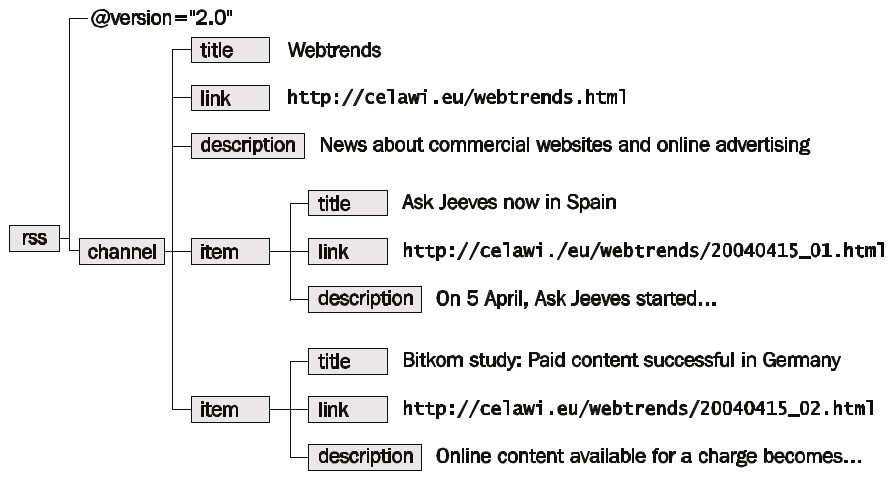
\includegraphics[scale=0.6]{structureRss}
	}
	\captionof{figure}{Estructura de un documento RSS simple como un diagrama de árbol}
	\source{fuente: \cite{wittenbrink2005rss}}
	\label{fig:Estructura de un documento RSS simple como un diagrama de árbol}
\end{minipage}

\subsection{Plataforma educativa LAEL}

En la figura \ref{fig:Suscriptor programa aprendizaje inglés básico}, se
muestra la acción de suscripción a una categoría (inglés básico) de un
usuario de sistema, con respecto al usuario tiene que iniciar sesión dentro
el sistema. 

\begin{minipage}{1.0\linewidth}
	\centering
	\fbox{
		
\includegraphics[scale=0.6]{basicEnglishSubscribe}
	}
	\captionof{figure}{Suscriptor programa aprendizaje inglés básico}
	\source{fuente: (Elaboración propia)}
	\label{fig:Suscriptor programa aprendizaje inglés básico}
\end{minipage}

En la figura \ref{fig:Presentación de un canal de noticia}, se muestra la
representación de un feed de la categoría inglés básico se utiliza un lector
desde la web. La estructura de un feed de noticia contempla título, fecha
para liberación y descripción.
 
\begin{minipage}{1.0\linewidth}
	\centering
	\fbox{
		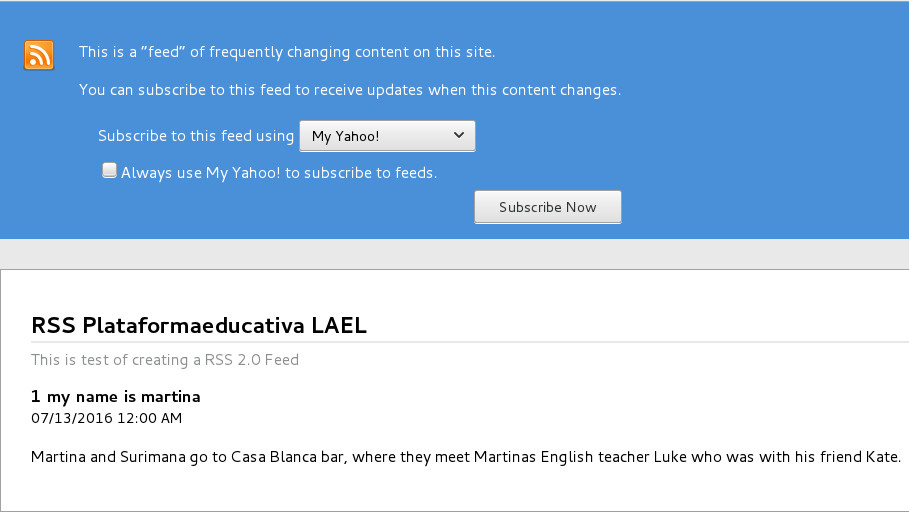
\includegraphics[scale=0.5]{basicEnglishRssFirefox}
	}
	\captionof{figure}{Presentación de un canal de noticia}
	\source{fuente: (Elaboración propia)}
	\label{fig:Presentación de un canal de noticia}
\end{minipage}

\section{El nuevo estándar atom}

Atom es otro tipo de feed compuesto por una serie de items
conocido como entry.

\subsection{Información básica de atom}

La estructura de un feed se describe a continuación.

\begin{itemize}

\item \textbf{title} contiene el título de la fuente de noticia.
\item \textbf{author} incluye información sobre el autor.
\item \textbf{updated} indica la última fecha de actualización.
\item \textbf{link} hace referencia a una versión diferente del contenido
y de la URI de atom.

\end{itemize}

La estructura de un entry se describe a continuación.

\begin{itemize}

\item \textbf{title} contiene el título de la fuente de noticia.
\item \textbf{summary} resumen del texto.
\item \textbf{updated} indica la última fecha de actualización.
\item \textbf{id} contiene una URI que identifica de forma única el feed.

\end{itemize}

En definitiva estos elementos son obligatorios de un elemento feed. Si esta
información no se encuentra presente un documento atom es considerado no
válido. \cite{wittenbrink2005rss}

En la figura \ref{fig:Estructura de un documento Atom}, se presenta la
estructura de un documento atom representado de forma gráfica.

\begin{minipage}{1.0\linewidth}
	\centering
	\fbox{
		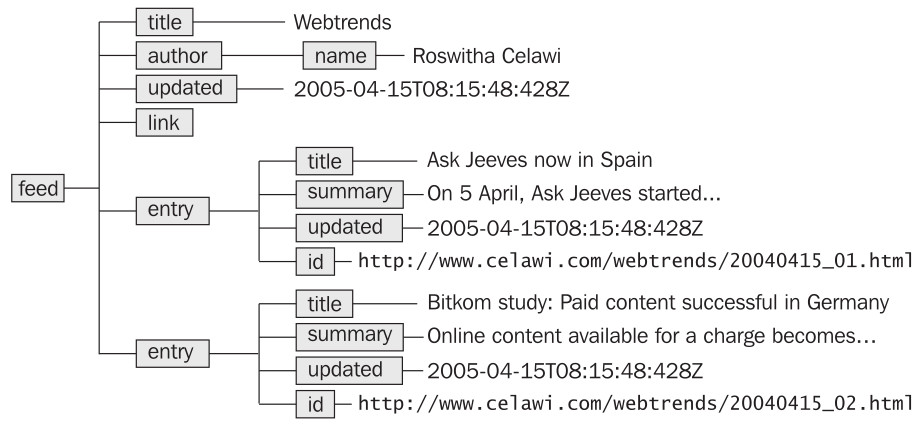
\includegraphics[scale=0.6]{structureAtom}
	}
	\captionof{figure}{Estructura de un documento Atom}
	\source{fuente: \cite{wittenbrink2005rss}}
	\label{fig:Estructura de un documento Atom}
\end{minipage}

\chapter{Aprendizaje Autorregulado propuesto por la Carrera LAEL}

\section{Autorregulado y aprendizaje autorregulado}

El aprendiz autorregulado se denomina a toda persona quien invierte su
tiempo en mejorar su conocimiento respecto a una lengua. Esta persona
realiza una planificación propia y autosugestiona su aprendizaje.

Ahora veamos lo que menciona Schunk(1997) la autorregulación en los
pensamientos, sentimientos y actos originados por los estudiantes que están
orientados sistemáticamente a la consecución de metas. Finalmente Zimmerman
(1994) define como el grado en el cual los individuos son participantes
activos en su propio proceso de aprendizaje desde el punto de vista
metacognitivo, motivación y relativo a su comportamiento. \cite{rinconconsideraciones}

\section{Descripción de la unidad patrocinadora}

La Carrera de LAEL lleva 35 años de trayectoria al
interior de la Facultad de Humanidades y Ciencias de la Educación, tuvo un
recorrido histórico, teniendo en cuenta las raíces que obtuvo
para su surgimiento en el año 1972, brindando materias de servicio dentro la
Facultad de Ciencias Puras y Naturales, en la Universidad Mayor de San Simón.
\cite{CMNPZ2014}

Actualmente en la Carrera de LAEL brinda servicios de enseñanza de lenguas,
traducción de documentos, planificación para las lenguas originarias y
extranjeras.

\subsection{Perfil profesional del estudiante en la Carrera LAEL}

En el año 2009, el estudiante de la Carrera LAEL, destacó el perfil
profesional constituido textualmente de la siguiente manera. \cite{Q2014}

\begin{itemize}

\item Un profesional comprometido con su medio en el que gracias a procesos de
investigación de la realidad boliviana aplicará métodos y técnicas
adecuados dentro del proceso de enseñanza aprendizaje de lenguas en el 
sistema educativo nacional y universitario.

\item Será capaz de evaluar y adaptar métodos de enseñanza, tanto para
las lenguas extranjeras como para el castellano y el quechua: lengua extranjera
y/o segunda lengua.

\item Realizar investigación multidisciplinaria para estudio e 
interpretación sobre:

	\begin{itemize}
		
	\item La enseñanza de las lenguas en el sistema educativo.
	\item Problemas de alfabetización en nuestro país, aportando desde la
	perspectiva de las lenguas.
	\item Problemas específicos de bilingüismo y de las relaciones entre 
	la lengua materna y la segunda lengua.
	\item Característica del castellano boliviano en sus diferentes niveles
	culturales.
	
	\end{itemize}
	
\item Investigar sobre las lenguas, realizando estudios comparativos de sistemas
de comunicación y estructuras de las lenguas en todos los niveles de 
enseñanza.

\item Evaluador de contenidos de las asignaturas relacionadas con el área de
lenguas en todos los niveles de enseñanza.

\item Desempeñar eficientemente en cualquier otro campo en el que exige 
conocimiento y formación de lenguas (Documento Carrera Lingüística 
Aplicada a la Enseñanza de lenguas 2009).

\end{itemize}

El perfil profesional del estudiante de la Carrera LAEL, señala que los
objetivos están enfocados en su mayoría en el área de técnicas que corroboran
al ámbito educativo a través de la enseñanza de las lenguas (L1 y L2). Este
documento esta vigente. \cite{Q2014}

\subsection{Objetivos profesionales}

A continuación se da a conocer los objetivos. EL licenciado de LAEL será capaz
de:

\begin{itemize}

\item Interpretar la actualidad de la educación nacional, particularmente en
la lingüística, proponiendo metodologías específicas para la enseñanza de la
lengua originaria y/o extranjera.
 
\item Analizar e interpretar la realidad educativa, regional y particularmente
la lingüística.

\item Proponer metodologías específicas para la enseñanza de la lengua
extranjera, del castellano y del quechua.

\item Planificar la enseñanza de las lenguas en los diferentes niveles de
enseñanza del sistema educativo nacional: inicial, primario, secundario y
universitario.

\item Evaluar, diseñar y/o adaptar material de apoyo para la enseñanza de
lenguas extranjeras.

\end{itemize}

A través de estos objetivos profesionales se desarrolla y facilita capacidades
en los estudiantes que favorecen su desenvolvimiento sin dificultad en el
ámbito laboral. \cite{CMNPZ2014}

\chapter{Desarrollo del Proyecto}

\section{Arquitectura cliente servidor}

Una arquitectura cliente servidor generalmente considerada como arquitectura
de sistema distribuido. Una vez más, un beneficio importante es la separación
e independencia de funcionalidad. \cite{sommerville2011software}

Esencialmente, el usuario final utiliza un navegador web para solicitar una
página esperando respuesta.

En la figura \ref{Una arquitectura cliente servidor para una filmoteca}, es un
ejemplo de un sistema en base al modelo cliente servidor. 
\cite{sommerville2011software}

\begin{figure}[!htb]
	\centering
	\fbox{
		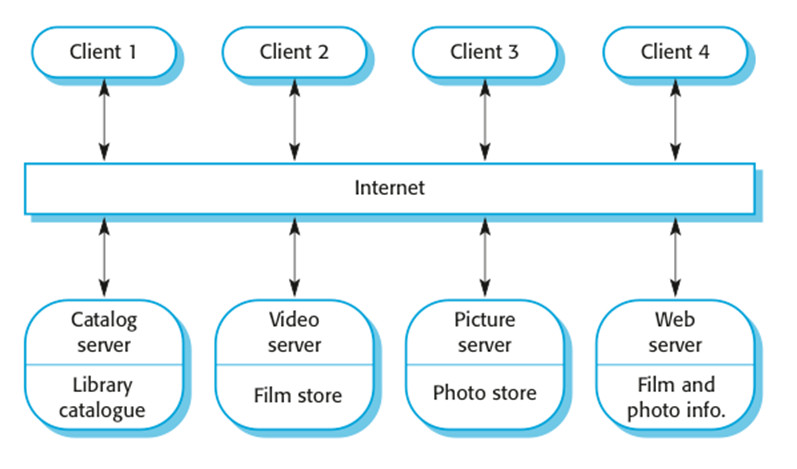
\includegraphics[scale=0.7]{architectureClientServer}
	}
	\caption{Una arquitectura cliente servidor para una filmoteca}
	\source{fuente: \cite{sommerville2011software}}
	\label{Una arquitectura cliente servidor para una filmoteca}
\end{figure}

\subsection{Patrón diseño: modelo vista controlador}

La idea de un patrón es una forma de presentar, compartir y reutilizar el
conocimiento sobre un sistema de software. Se piensa en un patrón
arquitectónico como una estilizada descripción abstracta de buena práctica,
que ha sido probada en diferentes sistemas y entornos. \cite{sommerville2011software}

En la figura \ref{fig:Arquitectura de aplicación web utilizando el patrón MVC},
se muestra una arquitectura de ejecución, cuando este patrón utiliza la
gestión en un sistema basado en la web. \cite{sommerville2011software}

\begin{minipage}{1.0\textwidth}
	\centering
	\fbox{
		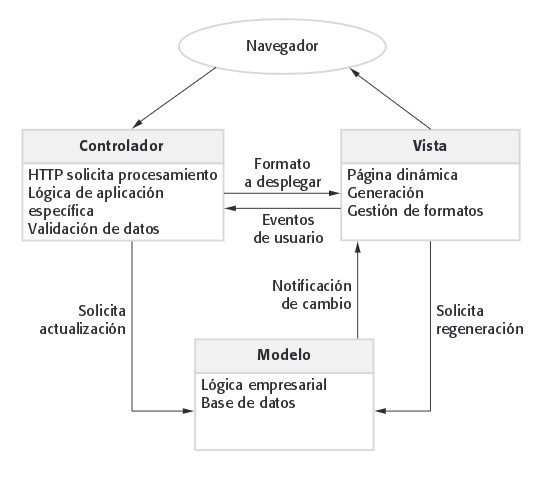
\includegraphics[scale=0.7]{mvcPattern}
	}
	\captionof{figure}{Arquitectura de aplicación web utilizando el patrón MVC}
	\source{fuente: \cite{sommerville2011software}}
	\label{fig:Arquitectura de aplicación web utilizando el patrón MVC}
\end{minipage}

\begin{itemize}

\item \textbf{Diseño del proyecto}

Se considera como patrón base de diseño Modelo Vista Controlador para realizar
la extension de funcionalidad de un Controlador representado como Administrador,
este Administrador realiza una abstracción y re uso de funcionalidad descrito
en la figura \ref{fig:Arquitectura extendida MVCA}.

\begin{minipage}{1.0\textwidth}
	\centering
	\fbox{
		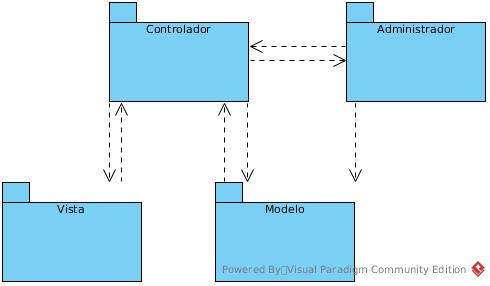
\includegraphics[scale=0.5]{mvcm}
	}
	\captionof{figure}{Arquitectura extendida MVCA}
	\source{fuente: (Elaboración propia)}
	\label{fig:Arquitectura extendida MVCA}
\end{minipage}

\end{itemize}

\section{Designación de rol}

En la plataforma web educativa se implementan cuatro tipos de roles.

\begin{itemize}

\item \textbf{Autorregulado}, rol designado a realizar suscripción o dar de
baja la misma.

\item \textbf{Tutor}, rol designado a un estudiante adscrito de la Carrera de
LAEL, quien tiene la posibilidad de crear podcast de tipo audio/vídeo, agregar
retro alimentación y agregar una transcripción. 

\item \textbf{Coordinador}, rol designado al docente de la Carrera de LAEL, quien
realiza la función de tutor y tiene la posibilidad de crear una categoría.

\item \textbf{Administrador}, rol designado a un adscrito de la Carrera de
Informática, quien tiene la posibilidad de gestionar la seguridad del sistema.

\end{itemize}

\section{Estructura de un podcast} \label{structPodcast}

Un podcast de tipo audio es representado como una estructura que contiene los
siguientes datos.

\begin{itemize}

\item \textbf{título}, nombre representativo, utilizado como identificador.
\item \textbf{imagen de portada}, imagen representativa.
\item \textbf{descripción}, resumen del tema.
\item \textbf{reproductor de audio}, grabación de diálogo.
\item \textbf{fecha de liberación}, fecha de publicación.
\item \textbf{historieta}, imagen de los personajes.
\item \textbf{transcripción}, texto del dialogo.
\item \textbf{actividad}, retro alimentación de actividad.
\item \textbf{resolución}, respuesta de actividad.
\item \textbf{glosario}, descripción de los términos.
\item \textbf{diccionario}, documento de referencia. 

\end{itemize}

Se describe la estructura de un podcast de tipo vídeo; con la diferencia de
tener: transcripción, actividad, resolución de actividad y glosario.

\begin{itemize}

\item \textbf{título}, nombre representativo, utilizado como identificador.
\item \textbf{imagen de portada}, imagen representativa.
\item \textbf{descripción}, resumen del tema.
\item \textbf{reproductor de vídeo}, uso de recursos: imagen, texto y audio.
\item \textbf{fecha liberación}, fecha de publicación.
\item \textbf{infografía}, imágenes descriptivas de tamaño pequeño.
\item \textbf{diccionario}, documento de referencia. 

\end{itemize}

\section{Definición de un componente}

Se considera el siguiente aspecto para describir el proceso de desarrollo.

\begin{itemize}

\item Tarjeta de historia de usuario.
\item Arquitectura de componente.
\item Modelo de componente.
\item Componente.
\item Implementar componente.
\item Problema/Solución de componente.

\end{itemize}

\section{\textquestiondown Cómo implementar un servicio agregado de noticia?} \label{serviceFeed}

La principal tarea de un servicio agregado de noticia es realizar la
notificación vía correo electrónico de nuevo contenido publicado en la web.

En la figura \ref{fig:Arquitectura job queue}, se muestra los componentes de
un servicio agregado de noticia y respectiva comunicación, un proceso en
segundo plano \footnote{segundo plano: Es un programa que se ejecuta sin
intervención del usuario. \cite{background}} se ejecuta respecto la fecha
de liberación descrito en la estructura de un podcast. sección
\ref{structPodcast}

\begin{minipage}{1.0\textwidth}
	\centering
	\fbox{
	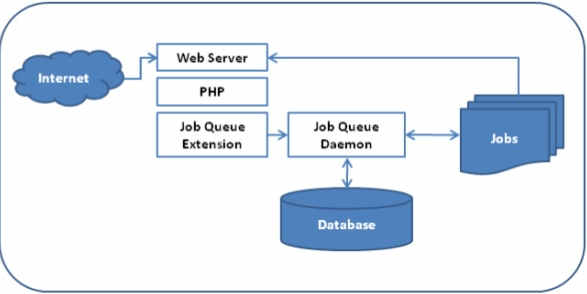
\includegraphics[scale=0.6]{jobQueue}
	}
	\captionof{figure}{Arquitectura job queue}
	\source{fuente:\cite{ossCamp2014}}
	\label{fig:Arquitectura job queue}
\end{minipage}

\subsection{Tarjeta de historia de usuario}

El equipo de informática realizó la elaboración de las historias respecto
a los deseos y sugerencias de un Coordinador de la Carrera de LAEL.

En particular deseo enfatizar los siguientes deseos a realizar:

\begin{itemize}

\item \textbf{Suscripción de usuario}, cuadros: \ref{Tarjeta historia de usuario 03},
\ref{Tarjeta historia de usuario 65}.
\item \textbf{Liberación de contenido}, cuadro: \ref{Tarjeta historia de usuario 58}.
\item \textbf{Baja de suscripción}, cuadro: \ref{Tarjeta historia de usuario 60}.

\end{itemize}

% add history card 03
\begin{minipage}[!htb]{\hsize}\centering
\begin{tabular}{|l|l|l|}
\hline
 & \textbf{Tarjeta Historia de Usuario} &  \\ \hline
ID Historia: 03 & \begin{tabular}[c]{@{}l@{}}Nombre: Suscripción a una\\ categoría.\end{tabular} & Fecha: 22/04/2014 \\ \hline
\multicolumn{3}{|l|}{Rol: Aprendiz autorregulado} \\ \hline
\begin{tabular}[c]{@{}l@{}}Modificación de historia\\ número: 05\end{tabular} & \begin{tabular}[c]{@{}l@{}}Iteración asignada: 7,8\end{tabular} & Prioridad en negocio: Medio \\ \hline
Tiempo estimado inicial: 20 & Riesgo en desarrollo: & Tipo de historia: Funcional \\ \hline
\multicolumn{3}{|l|}{\begin{tabular}[c]{@{}l@{}}Descripción:\\ \\ Yo como usuario aprendiz autorregulado deseo suscribirme a un determinado lenguaje \\ (francés básico, ingles básico, quechua básico, quechua psicosocial, fonética quechua), \\tal que me beneficie en recibir notificación de nuevo contenido vía correo. \\ Para esto ya no necesito ingresar mi correo electrónico.\end{tabular}} \\ \hline
\multicolumn{3}{|l|}{\begin{tabular}[c]{@{}l@{}}Pre condición:	\\ \\ Contenido publicado. \\ Servidor SMTP externo configurado.\\ Configuración de credenciales en sistema con servidor SMTP.\end{tabular}} \\ \hline
\multicolumn{3}{|l|}{\begin{tabular}[c]{@{}l@{}}Post condición:\\ \\ Recibir un mensaje en mi bandeja de entrada de mi cuenta de correo.\end{tabular}} \\ \hline
\multicolumn{3}{|l|}{\begin{tabular}[c]{@{}l@{}}Actividades:\\ \\ Desplegar lista de categorías para suscripción.\\ Permitir al usuario seleccionar de la lista de categoría para suscribirse. \\ Guardar suscripción de usuario y registrar fecha.\end{tabular}} \\ \hline
\multicolumn{3}{|l|}{\begin{tabular}[c]{@{}l@{}}Observaciones:\\ \\ La suscripción permite acceder a las noticias de nuevos contenidos de categoría.\end{tabular}} \\ \hline
\begin{tabular}[c]{@{}l@{}}.....................................................\\ Msc. Lic. Vladimir Costas Juaregui\\ PROJECT MANAGER\end{tabular} & \begin{tabular}[c]{@{}l@{}}..........................................\\ Lic. Manuel Camacho Arce\\ PRODUCT OWNER\end{tabular} & \begin{tabular}[c]{@{}l@{}}.........................................\\ Juan Omar Huanca Balboa\\ SCRUM MASTER\end{tabular} \\ \hline
\end{tabular}
\captionof{table}{Tarjeta historia de usuario 03}
\source{fuente: (Elaboración propia)}
\label{Tarjeta historia de usuario 03}
\end{minipage}

% add history card 65
\begin{minipage}[!htb]{\hsize}\centering
\begin{tabular}{|l|l|l|}
\hline
 & \textbf{Tarjeta Historia de Usuario} &  \\ \hline
ID Historia: 65 & \begin{tabular}[c]{@{}l@{}}Nombre: Suscripción a una\\ categoría por red social.\end{tabular} & Fecha: 29/08/2016 \\ \hline
\multicolumn{3}{|l|}{Rol: Aprendiz autorregulado} \\ \hline
\begin{tabular}[c]{@{}l@{}}Modificación de historia\\ número: \end{tabular} & \begin{tabular}[c]{@{}l@{}}Iteración asignada: 9, 11\end{tabular} & Prioridad en negocio: Medio \\ \hline
Tiempo estimado inicial: 20 & Riesgo en desarrollo: & Tipo de historia: Funcional \\ \hline
\multicolumn{3}{|l|}{\begin{tabular}[c]{@{}l@{}}Descripción:\\ \\ Yo como usuario aprendiz autorregulado deseo suscribirme a un determinado lenguaje \\ (francés básico, ingles básico, quechua básico, quechua psicosocial, fonética quechua), \\tal que me beneficie en recibir notificación de nuevo contenido vía correo.\\ Para esto necesito pinchar sobre un botón de red social: facebook, google, twitter.\end{tabular}} \\ \hline
\multicolumn{3}{|l|}{\begin{tabular}[c]{@{}l@{}}Pre condición:	\\ \\ Contenido publicado. \\ Usuario autentificado por red social: facebook, google, twitter. \\ Realizar configuración de sistema con en servidor externo: facebook, google, twitter.\end{tabular}} \\ \hline
\multicolumn{3}{|l|}{\begin{tabular}[c]{@{}l@{}}Actividades:\\ \\ Desplegar lista de categorías para suscripción.\\ Permitir al usuario seleccionar de la lista de categoría para suscribirse. \\ Guardar suscripción de usuario y registrar fecha.\end{tabular}} \\ \hline
\multicolumn{3}{|l|}{\begin{tabular}[c]{@{}l@{}}Observaciones:\\ \\ La suscripción permite acceder a las noticias de nuevos contenidos de categoría.\end{tabular}} \\ \hline
\begin{tabular}[c]{@{}l@{}}.....................................................\\ Msc. Lic. Vladimir Costas Juaregui\\ PROJECT MANAGER\end{tabular} & \begin{tabular}[c]{@{}l@{}}..........................................\\ Lic. Manuel Camacho Arce\\ PRODUCT OWNER\end{tabular} & \begin{tabular}[c]{@{}l@{}}.........................................\\ Juan Omar Huanca Balboa\\ SCRUM MASTER\end{tabular} \\ \hline
\end{tabular}
\captionof{table}{Tarjeta historia de usuario 65}
\source{fuente: (Elaboración propia)}
\label{Tarjeta historia de usuario 65}
\end{minipage}

% add user history card 58
\begin{minipage}[!htb]{\hsize}\centering
\begin{tabular}{|l|l|l|}
\hline
 & \textbf{Tarjeta Historia de Usuario} &  \\ \hline
ID Historia: 58 & \begin{tabular}[c]{@{}l@{}}Nombre: Liberación \\ de contenido\end{tabular} & Fecha: 03/05/2015 \\ \hline
\multicolumn{3}{|l|}{Rol: Tutor} \\ \hline
\begin{tabular}[c]{@{}l@{}}Modificación de historia\\ número:\end{tabular} & Iteración asignada: 10 & Prioridad en negocio: Medio \\ \hline
Tiempo estimado inicial: 35 & Riesgo en desarrollo: & Tipo de historia: Funcional \\ \hline
\multicolumn{3}{|l|}{\begin{tabular}[c]{@{}l@{}}Descripción:\\ \\ Yo como usuario tutor deseo realizar la automática publicación de mi contenido tal que se \\ publiquen de acuerdo a fecha indicada en el registro.\end{tabular}} \\ \hline
\multicolumn{3}{|l|}{\begin{tabular}[c]{@{}l@{}}Pre condición:	\\ \\ Usuario autentificado. \\Contenido registrado. \\ Fecha actual de sistema debe ser mayor a fecha de liberación de contenido.\end{tabular}} \\ \hline
\multicolumn{3}{|l|}{\begin{tabular}[c]{@{}l@{}}Actividades: \\ \\ Generar un script para obtener los contenidos inhabilitados \\ Enviar un mensaje de notificación a los usuarios suscritos a categoría respectiva.\\ Cambiar estado de contenido en habilitado.\end{tabular}} \\ \hline
\multicolumn{3}{|l|}{\begin{tabular}[c]{@{}l@{}}Observaciones:\\ \\ La liberación de contenido debe estar condicionado a fecha de liberación.\end{tabular}} \\ \hline
\begin{tabular}[c]{@{}l@{}}.....................................................\\ Msc. Lic. Vladimir Costas Juaregui\\ PROJECT MANAGER\end{tabular} & \begin{tabular}[c]{@{}l@{}}..........................................\\ Lic. Manuel Camacho Arce\\ PRODUCT OWNER\end{tabular} & \begin{tabular}[c]{@{}l@{}}.........................................\\ Juan Omar Huanca Balboa\\ SCRUM MASTER\end{tabular} \\ \hline
\end{tabular}
\captionof{table}{Tarjeta historia de usuario 58}
\source{fuente: (Elaboración propia)}
\label{Tarjeta historia de usuario 58}
\end{minipage}

% add user history card 60
\begin{minipage}[!htb]{\hsize}\centering
\begin{tabular}{|l|l|l|}
\hline
 & \textbf{Tarjeta Historia de Usuario} &  \\ \hline
ID Historia: 60 & \begin{tabular}[c]{@{}l@{}}Nombre: Dar de baja \\ suscripción.\end{tabular} & Fecha: 19/05/2015 \\ \hline
\multicolumn{3}{|l|}{Rol: Aprendiz autorregulado} \\ \hline
\begin{tabular}[c]{@{}l@{}}Modificación de historia\\ número: 04\end{tabular} & Iteración asignada: 11 & Prioridad en negocio: Bajo \\ \hline
Tiempo estimado inicial: 15 & Riesgo en desarrollo: & Tipo de historia: Funcional \\ \hline
\multicolumn{3}{|l|}{\begin{tabular}[c]{@{}l@{}}Descripción:\\ \\ Yo como usuario aprendiz autorregulado deseo dar de baja mi suscripción a un determinada \\ categoría tal que me beneficie no recibir más notificación.\\ Para esto necesito pinchar sobre el botón lado la categoría.\end{tabular}} \\ \hline
\multicolumn{3}{|l|}{\begin{tabular}[c]{@{}l@{}}Pre condición:\\ \\ Usuario autentificado. \\ Usuario suscrito\end{tabular}} \\ \hline
\multicolumn{3}{|l|}{\begin{tabular}[c]{@{}l@{}}Post condición:\\ \\ Dejar de recibir notificación a bandeja de correo.\end{tabular}} \\ \hline
\multicolumn{3}{|l|}{\begin{tabular}[c]{@{}l@{}}Actividades:\\ \\ Desplegar la lista de categorías.\\ Verificar registro de categoría.\\ Eliminar registro de suscripción.\\Cambiar estado de suscripción y registrar fecha de baja.\end{tabular}} \\ \hline
\begin{tabular}[c]{@{}l@{}}.....................................................\\ Msc. Lic. Vladimir Costas Juaregui\\ PROJECT MANAGER\end{tabular} & \begin{tabular}[c]{@{}l@{}}..........................................\\ Lic. Manuel Camacho Arce\\ PRODUCT OWNER\end{tabular} & \begin{tabular}[c]{@{}l@{}}.........................................\\ Juan Omar Huanca Balboa\\ SCRUM MASTER\end{tabular} \\ \hline
\end{tabular}
\captionof{table}{Tarjeta historia de usuario 60}
\source{fuente: (Elaboración propia)}
\label{Tarjeta historia de usuario 60}
\end{minipage}

\subsection{Arquitectura de componente}

\begin{itemize}

\item \textbf{Suscripción y baja de suscripción}
en la figura \ref{fig:Diagrama de caso de uso para personalizar suscripción, dar baja},
las acciones del rol autorregulado realiza el requerimiento descrito en cuadro
\ref{Tarjeta historia de usuario 03}, cuadro 
\ref{Tarjeta historia de usuario 65} y cuadro
\ref{Tarjeta historia de usuario 60}.

\begin{minipage}{1.0\textwidth}
	\centering
	\fbox{
		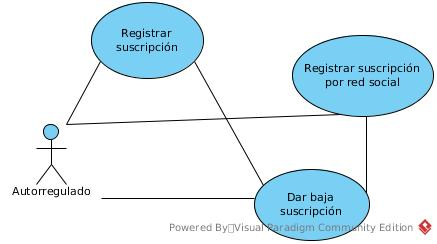
\includegraphics[scale=0.6]{useCaseSubscription}
	}
	\captionof{figure}{Diagrama de caso de uso para personalizar suscripción, dar baja}
	\source{fuente: (Elaboración propia)}
	\label{fig:Diagrama de caso de uso para personalizar suscripción, dar baja}
\end{minipage}

\item \textbf{Liberación de contenido} en la figura 
\ref{fig:Diagrama de caso de uso para liberación de contenido}, la acción del
rol tutor realiza la definición de fecha de liberación y el proceso cron
ejecuta el script descrito en cuadro \ref{Tarjeta historia de usuario 58}.

\begin{minipage}{1.0\textwidth}
	\centering
	\fbox{
		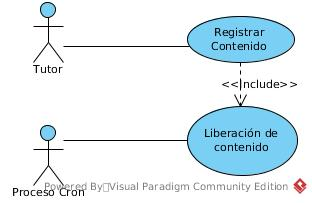
\includegraphics[scale=0.7]{useCaseRelease}
	}
	\captionof{figure}{Diagrama de caso de uso para liberación de contenido}
	\source{fuente: (Elaboración propia)}
	\label{fig:Diagrama de caso de uso para liberación de contenido}
\end{minipage}

\item \textbf{Suscripción, baja de suscripción y liberación de contenido}
en la figura \ref{fig:Diagrama de clase para suscriptor}, el diagrama
representa la composición de datos y comunicación de las clases.

\begin{minipage}{1.0\textwidth}
	\centering
	\fbox{
		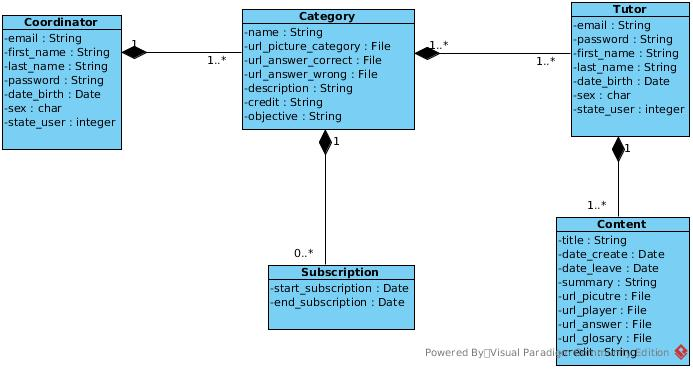
\includegraphics[scale=0.6]{classSubscription}
	}
	\captionof{figure}{Diagrama de clase para suscriptor}
	\source{fuente: (Elaboración propia)}
	\label{fig:Diagrama de clase para suscriptor}
\end{minipage}

\item \textbf{Suscripción y baja de suscripción}
en la figura \ref{fig:Diagrama de secuencia para suscripción}, el diagrama
de secuencia representa la comunicación del rol autorregulado con las
diferentes clases.

\begin{minipage}{1.0\textwidth}
	\centering
	\fbox{
		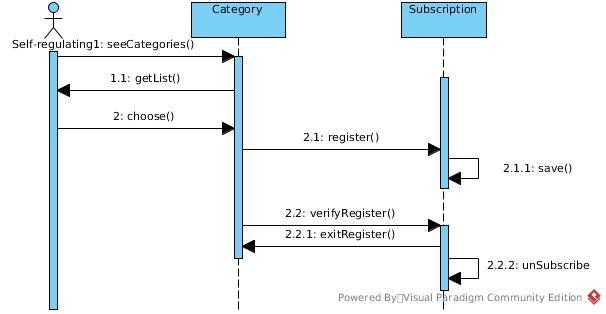
\includegraphics[scale=0.7]{sequenceSubscription}
	}
	\captionof{figure}{Diagrama de secuencia para suscripción}
	\source{fuente: (Elaboración propia)}
	\label{fig:Diagrama de secuencia para suscripción}
\end{minipage}

\item \textbf{Liberación de contenido}
en la figura \ref{fig:Diagrama de secuencia para liberación de contenido},
el diagrama de secuencia representa la comunicación del rol tutor con las
diferentes clases, el proceso cron verifica el registro de contenido para
luego ejecutar un script.

\begin{minipage}{1.0\textwidth}
	\centering
	\fbox{
		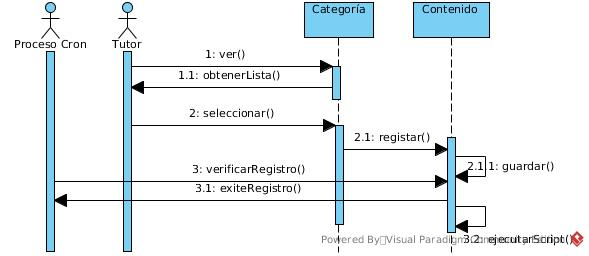
\includegraphics[scale=0.7]{sequenceRelease}
	}
	\captionof{figure}{Diagrama de secuencia para liberación de contenido}
	\source{fuente: (Elaboración propia)}
	\label{fig:Diagrama de secuencia para liberación de contenido}
\end{minipage}

\end{itemize}

\subsection{Modelo de componente}

\begin{itemize}

\item \textbf{Suscripción y baja de suscripción}
en la figura \ref{fig:Modelo de datos para suscriptor}, el modelo de datos
representa la persistencia de suscripción de categoría y suscripción por
red social.

\begin{minipage}{1.0\textwidth}
	\centering
	\fbox{
		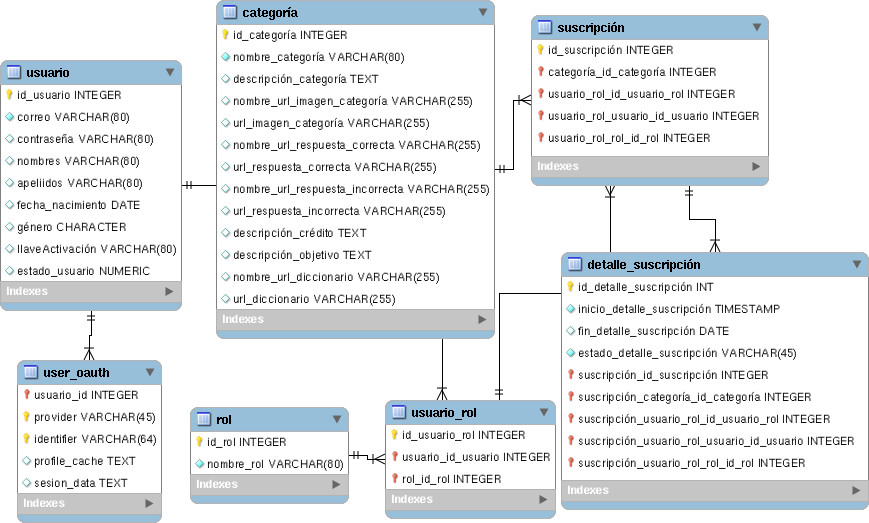
\includegraphics[scale=0.5]{modelSubscription}
	}
	\captionof{figure}{Modelo de datos para suscriptor}
	\source{fuente: (Elaboración propia)}
	\label{fig:Modelo de datos para suscriptor}
\end{minipage}

\item \textbf{Liberación de contenido}
en la figura \ref{fig:Modelo de datos para liberación de contenido},
el modelo de datos representa la persistencia de registro de contenido
y fecha de liberación.

\begin{minipage}{1.0\textwidth}
	\centering
	\fbox{
		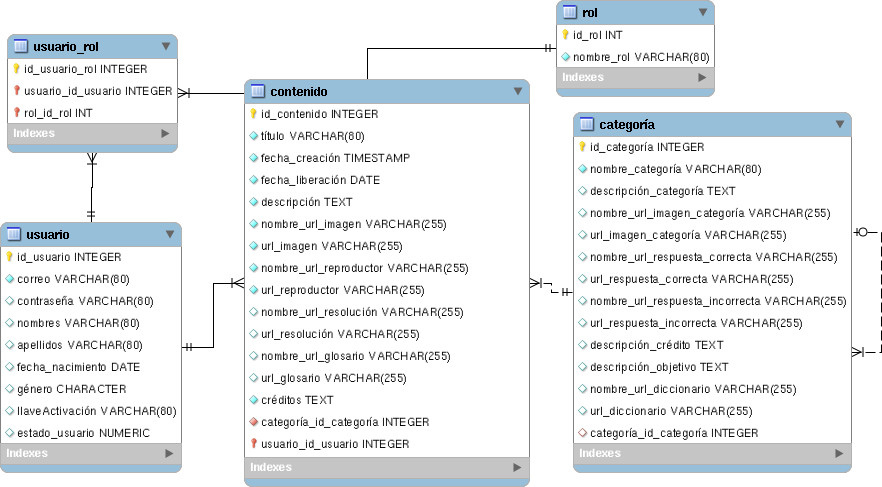
\includegraphics[scale=0.5]{modelRelease}
	}
	\captionof{figure}{Modelo de datos para liberación de contenido}
	\source{fuente: (Elaboración propia)}
	\label{fig:Modelo de datos para liberación de contenido}
\end{minipage}

La suscripción conformado por categoría genera una bitácora \footnote{bitácora:
Mecanismo persistencia de actividades en el tiempo. (Elaboración propia)}
y detalle\textunderscore suscripción.

\end{itemize}

\subsection{Componente}

\begin{itemize}

\item \textbf{Suscripción de usuario}
se propone dos opciones para realizar una suscripción.

\begin{itemize}

\item \textbf{Manual}, permite realizar la suscripción con una dirección de
correo sujeto a verificación de sistema.

\item \textbf{Token de red social}, permite realizar la suscripción con un
servicio externo provisto por redes sociales de google, facebook y twitter.

\end{itemize}

\textbf{Manual} en la figura \ref{fig:Ventana emergente de suscripción}, se
representa un formulario de registro de dirección de correo electrónico para
realizar una suscripción. 

\begin{minipage}{1.0\textwidth}
	\centering
	\fbox{
		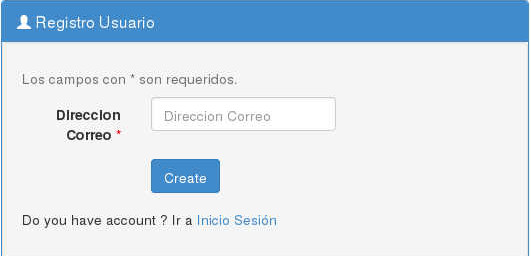
\includegraphics[scale=0.7]{modalSubscribe}
	}
	\captionof{figure}{Ventana emergente de suscripción}
	\source{fuente: (Elaboración propia)}
	\label{fig:Ventana emergente de suscripción}
\end{minipage}

\textbf{Token \footnote{Token: Se clasifica como una de las cinco clases de
fichas que describen sus funciones (constantes, identificadores, operadores,
palabras reservadas y separadores) de acuerdo con las reglas del lenguaje de
programación. \cite{token}} de red social} en la figura \ref{fig:Formulario
de inicio de sesión}, el formulario de inicio de sesión tiene la funcionalidad
de ingresar a su entorno de trabajo.

\begin{minipage}{1.0\textwidth}
	\centering
	\fbox{
		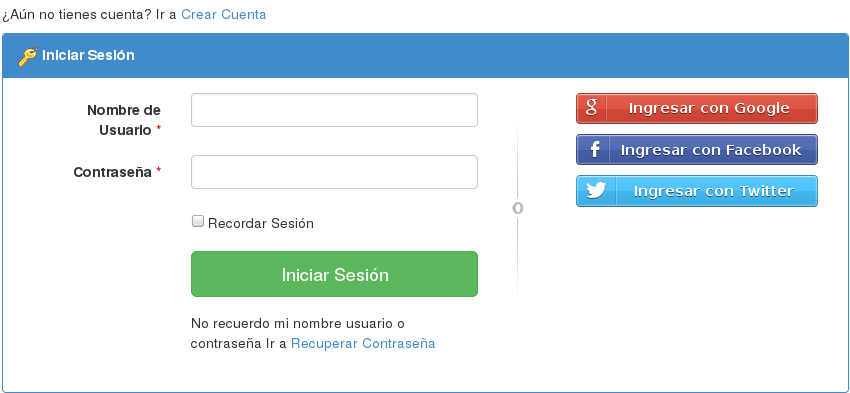
\includegraphics[scale=0.6]{login}
	}
	\captionof{figure}{Formulario de inicio de sesión}
	\source{fuente: (Elaboración propia)}
	\label{fig:Formulario de inicio de sesión}
\end{minipage}

\begin{enumerate}

\item \textbf{Facebook}, en la figura \ref{fig:Aplicación de sesión para facebook},
el flujo en un servidor de facebook para realizar el acceso de una cuenta válida.

\begin{minipage}{1.0\textwidth}
	\centering
	\fbox{
		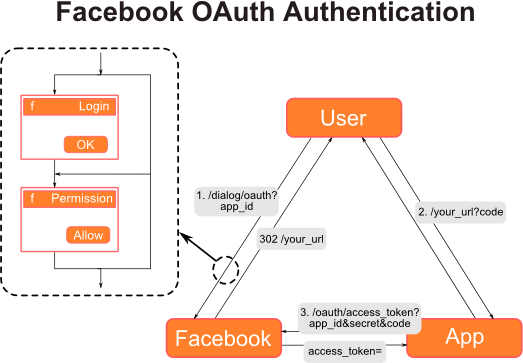
\includegraphics[scale=0.5]{oauthFacebook}
	}
	\captionof{figure}{Aplicación de sesión para facebook}
	\source{fuente: \cite{oauthFacebook}}
	\label{fig:Aplicación de sesión para facebook}
\end{minipage}

\item \textbf{Google}, en la figura \ref{fig:Aplicación de sesión para google}, el
diagrama secuencia facilita el acceso para una cuenta válida de un usuario.

\begin{minipage}{1.0\textwidth}
	\centering
	\fbox{
		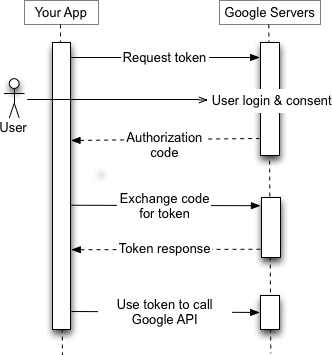
\includegraphics[scale=0.7]{oauth20Google}
	}
	\captionof{figure}{Aplicación de sesión para google}
	\source{fuente: \cite{oauthGoogle}}
	\label{fig:Aplicación de sesión para google}	
\end{minipage}

\item \textbf{Twitter}, en la figura \ref{fig:Aplicación de sesión para twitter},
el flujo dentro un servidor de twitter permite realizar el inicio de sesión de
una cuenta de usuario.

\begin{minipage}{1.0\textwidth}
	\centering
	\fbox{
		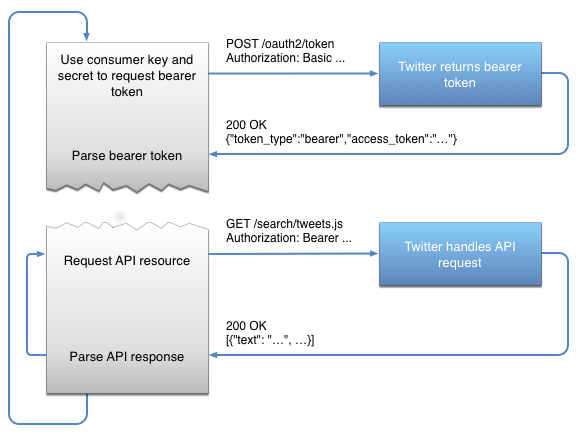
\includegraphics[scale=0.5]{oauth10Twitter}
	}
	\captionof{figure}{Aplicación de sesión para twitter}
	\source{fuente: \cite{oauthTwitter}}
	\label{fig:Aplicación de sesión para twitter}
\end{minipage}

\end{enumerate}

\item \textbf{Baja suscripción} en la figura 
\ref{fig:Suscripción programa aprendizaje francés básico}, un usuario de
sistema suscrito a una categoría (francés básico) desea dar de baja su
respectiva suscripción. Para el mismo solo se tiene que pinchar sobre el botón
\textquotedouble{Suscrito}. 

\begin{minipage}{1.0\linewidth}
	\centering
	\fbox{
		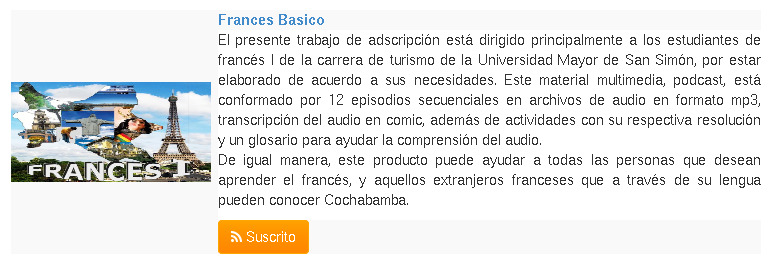
\includegraphics[scale=0.6]{basicFranceSubscribed}
	}
	\captionof{figure}{Suscripción programa aprendizaje francés básico}
	\source{fuente: (Elaboración propia)}
	\label{fig:Suscripción programa aprendizaje francés básico}
\end{minipage}

\item \textbf{Liberación de contenido} en la figura
\ref{fig:Formulario registro de contenido}, el formulario de registro de
contenido permite definir la fecha de liberación del propio contenido.

\begin{minipage}{1.0\linewidth}
	\centering
	\fbox{
		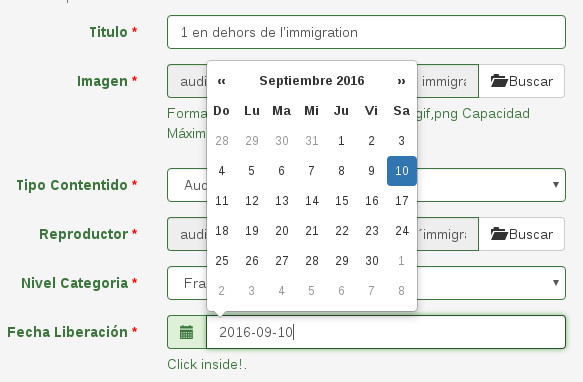
\includegraphics[scale=0.7]{formContent}
	}
	\captionof{figure}{Formulario registro de contenido}
	\source{fuente: (Elaboración propia)}
	\label{fig:Formulario registro de contenido}
\end{minipage}

\end{itemize}
	
\subsection{Implementar componente}

\begin{itemize}

\item \textbf{Suscripción de usuario - implementar en el servidor} el
siguiente segmento de código permite personalizar la suscripción por
categoría, el suscriptor obtiene las categorías habilitadas. 

\begin{lstlisting}[language=PHP, caption={Personalización de suscriptor.}]
public function actionCustomRss($idCategory) {
    ob_end_clean();
    header('Content-type: text/xml; charset=utf-8');
    $this->layout = false;    // turn off layout
    $criteria = new CDbCriteria;     // add custom criteria
    $criteria->addCondition('t.category_id_category=:Column1');
    $criteria->addCondition('t.category_id_category in (select i.category_id_category
    from interest as i) and t.content_status=' . Yii::app()->params[
    'stateContentAvailable']);
    $criteria->select = 't.title,t.summary,t.date_leave';
    $criteria->params = array(':Column1' => $idCategory);
    $data = Content::model()->findAll($criteria);
    $this->renderPartial('_viewItemChannel', array(
        'data' => $data,
    ));     // redirect view
}
\end{lstlisting}

En la linea dos tiene la funcionalidad limpiar buffer de salida y
des habilitar su uso.

En la linea tres agrega la cabecera de un documento XML y codificación con
el formato UTF-8 \footnote{UTF-8: El estándar Unicode cubre todos
los caracteres, signos de puntuación y símbolos en el mundo. Unicode 
procesamiento, almacenamiento y transporte de texto, independiente de la 
plataforma y lenguaje \cite{utf8}}.

\item \textbf{Baja de suscripción - implementar en el servidor} el siguiente
segmento de código verifica el registro de una suscripción, si la verificación
es verdadera realiza la baja, caso contrario registra nueva suscripción.

\begin{lstlisting}[language=PHP, caption={Verificación registro suscripción.}]
public function actionVerifySubscribeCategory() {
$user_id_user = Yii::app()->user->id; // get user id
...
foreach ($model_user_rols as $model_user_rol) { // iterate each row UserRol
    ...
    $model_subscription = Subscription::model()->findByAttributes(array(
    'category_id_category' => $category_id_category, 'id_user_rol' => 
    $id_user_rol, 'rol_id_rol' => $rol_id_rol, 'user_id_user' => $user_id_user));
    $manager_detail_subscription = new DetailSubscriptionManager();
    if ($model_subscription == null) { // verify array is null
        $model_subscription = new Subscription('create'); // new model Interest
        ...
        if ($model_subscription->validate()) { // verify valitation
            $this->saveModel($model_subscription); // save tuple
            ...
        }
    } else {
        $model_detail_subscription = DetailSubscription::model()->findByAttributes
        (array('subscription_id_subscription' => $model_subscription->
        id_subscription, 'subscription_category_id_category' => 
        $category_id_category, 'subscription_user_id_user' => $user_id_user,
        'status_detail_subscription' => Yii::app()->params[
        'stateDetailSubscribeAvailable']));
        if ($model_detail_subscription == null) { // verify change
            ...
        }
    }
}    
}
\end{lstlisting}

\item \textbf{Liberación de contenido - implementar en el servidor} el
proceso cron utiliza una tabla para la definición para una tarea, la
instrucción realiza ejecución de un script para liberación de diferentes
podcasts.

Ejecutar el comando sobre una terminal. A continuación se debe iniciar sesión
como usuario \textquotedouble{root}.

\begin{lstlisting}[language=bash, caption={Acceso archivo crontab.}]
# contrab -e
\end{lstlisting}

\textbf{sobre una sola línea} el comando a ejecutar tiene la siguiente sintaxis
de minuto (0-59) hora (0-23) día del mes (1-31) mes del año (1-12) día de la
semana (0-7) comando/script/tarea a ejecutar.

\begin{lstlisting}[language=bash, caption={Comando para ejecución de tarea.}]
0 0 * * * php /var/www/html/plataformaeducativalael/protected/utils/job.php job
\end{lstlisting}

A continuación la función principal del script job.php, obtiene podcast
a ser liberado. Enviar una notificación por correo a los usuarios suscritos.

\begin{lstlisting}[language=PHP, caption={Método principal de clase JobCommand.}]
public function run($args) {
    $jobs = $this->getJobs();
    foreach ($jobs as $job) {
        Yii::log("Running - Job [". $job->title ."] scheduled for ".
        $job->date_create, 'info', 'jobprocessor');
        $job->content_status = Yii::app()->params['stateContentAvailable'];
        $job->save(); // save data
        $this->sendMailSubscribed($job->category_id_category, $job->user_id_user,
        $job->title, $job->summary);
    }
}
\end{lstlisting}

\end{itemize}

\subsection{Problema/Solución de componente}

\begin{itemize}

\item \textbf{Suscripción de usuario} la dificultad surgió para implementar.

\begin{itemize}

\item Generación única de modal \footnote{modal: Una ventana modal es,
por tanto, normalmente una ventana secundaria. El usuario tiene interarticular
con el antes de que el control se pueda devolver a la solicitud principal.
\cite{modal}} para cada categoría.

\end{itemize}

La ventana modal utiliza el identificador de la categoría hija, para una lista
de categorías hijas pinchar sobre el botón de la ultima categoría realiza la
replica de identificador sobre los demás elementos.

\begin{enumerate}

\item \textbf{Generar único identificador por modal - implementar en el cliente}
como mecanismo de solución se generara un identificador conformado por
categoría padre y categoría hija.

\begin{lstlisting}[language=HTML, caption={Generador ventana modal.}]
<?php $this->beginWidget(
        'booster.widgets.TbModal', array(
    'id' => 'myModal' . $category_id,
));?>
<div class="modal-body">
    <div class="panel-body">
        <?php $this->renderPartial('//site/createRegisterSuscribe', 
        array('model_user' => $model_user)); ?>
    </div>
</div>
<?php $this->endWidget(); ?>
\end{lstlisting}

El problema de notificación vía correo electrónico se genera por las etiquetas
propias de HTML \footnote{HTML: Es el conjunto de símbolos de marcado o
códigos insertados en un archivo destinado a la visualización de una página
web mundial. \cite{html}}.

\end{enumerate}

\item \textbf{Baja de suscripción} la dificultad se obtuvo al momento de implementar.

\begin{itemize}

\item Estado usuario botón suscripción.

\end{itemize}

\begin{enumerate}

\item \textbf{Estado usuario botón suscripción - implementar en el cliente}
en el segmento de código se utiliza una variable local para almacenar el valor
de una categoría suscrita y realizar el cambio según la verificación de registro
de usuario.

\begin{lstlisting}[language=PHP, caption={Cambio de estado botón de suscripción.}]
$category_id_result = 0;
foreach ($model_detail_subscriptions as $model_detail_subscription){
    if ($model_detail_subscription->subscription_category_id_category ==
            $category_id){
        $category_id_result = $category_id;
    }
}
$this->widget(
'booster.widgets.TbButton', array(
'label' => ($category_id_result == $category_id) ?'<i class="fa fa-rss"></i> '.
    Yii::t('app', 'Subscribed') :'<i class="fa fa-rss"></i> '. Yii::t('app', 
    'Subscribe'),
'context' => 'warning',
'encodeLabel'=>false,        
'htmlOptions' => array(
    'id' => 'button' . $category_id,
    'data-dismiss' => 'modal',
    'class'=>'btn-subscribe',
    'ajax' => array(
        'type' => 'POST',
        'url' => $this->createUrl('subscription/verifySubscribeCategory'),
        'success' => 'js:function(data){ $("#button' . $category_id . '").html("'
        . Yii::t("app", "Subscribed") . '");}',
        'data' => array(
            'idCategory' => 'js:$("#user-formRegisterSuscribe' . $category_id 
                . ' #User_category_id").val()',
        ),
    ),
),
'encodeLabel' => false)
);
\end{lstlisting}

\end{enumerate}

\item \textbf{Liberación de contenido}

\begin{itemize}

\item Envió de mensaje de notificación.
\item Obtener contenido sujeto a condición de liberación. 

\end{itemize}

\begin{enumerate}

\item \textbf{Envió de mensaje - implementar en el servidor}

El segmento de código implementa el envió de correo, tiene la característica
de mostrar un mensaje sin página maestra.

\begin{lstlisting}[language=PHP, caption={Envió de mensaje sin  contenedor de página.}]
private function sendMailSubscribed($idCategory, $idUser, $title, $summary) {
$userRols = Category::model()->getRecentUserSubscribe($idCategory);
foreach ($userRols->categoryUserRol as $userRol) {
    if ($idUser != $userRol->user_id_user) {
        $subject = Yii::app()->params['setSubjectContentRelease'];
        $body = Yii::app()->params['setBodyContentRelease'] . $title . $summary
        . Yii::app()->params['setBodyBelowContentRelease'] 
        . Yii::app()->params['adminEmail']
        . Yii::app()->params['setBodyBottomContentRelease'];
        $to = $userRol->userIdUser->email;
        $mail = new YiiMailer(); // send mail
        $mail->setBody($body); //use cron view from views/mail
        $mail->setData(array('message' => $subject, 'name' => get_class($this), 
        'description' => 'Cron job', 'mailer' => $mail));
        $mail->render(); //render HTML mail, layout is set from config file
        $mail->From = Yii::app()->params['adminEmail'];
        $mail->FromName = Yii::app()->params['fromNameConsole'];
        $mail->Subject = $subject;
        $mail->AddAddress($to);
        if ($mail->send()) { // send
            Yii::log(Yii::app()->params['succeedSendContentRelease']); 
        } else {
            Yii::log(Yii::app()->params['wrongSendContenRelease']);
        }
    }
}
}
\end{lstlisting}

\item \textbf{Obtención de contenido - implementar en el servidor}
en el segmento de código se realiza el uso de la función \textquotedouble{scopes}
para obtener contenido habilidad y la fecha de sistema es mayor la fecha
de liberación.

\begin{lstlisting}[language=PHP, caption={Obtención de contenido para liberar podcast.}]
public function scopes() {
return array(
    'active' => array(
        'condition' => 'content_status='.Yii::app()->params[
            'stateContentUnavailable'],
    ),
    'current' => array(
        'condition' => 'date_leave < now()',
    ),
);
}
\end{lstlisting}

\end{enumerate}

\end{itemize}

\section{\textquestiondown Cómo implementar un glosario y subtitulado?}

Relacionar un reproductor de podcast de tipo audio con su transcripción
genera un efecto de subtitulado. 

Definir un glosario de términos con significado.
 
\subsection{Tarjeta de historia de usuario}

El equipo de informática realizó la elaboración de las historias respecto
a los deseos y sugerencias de un Coordinador de la Carrera de LAEL.

En particular deseo enfatizar los siguientes deseos a realizar:

\begin{itemize}

\item \textbf{Gestionar glosario de podcast}, cuadro
\ref{Tarjeta historia de usuario 64}.
\item \textbf{Gestionar subtitulado de podcast audio}, cuadro 
\ref{Tarjeta historia de usuario 66}.

\end{itemize}

% add user history card 64
\begin{minipage}[!htb]{\hsize}\centering
\begin{tabular}{|l|l|l|}
\hline
 & \textbf{Tarjeta Historia de Usuario} &  \\ \hline
ID Historia: 64 & \begin{tabular}[c]{@{}l@{}}Nombre: Registrar\\ glosario audio podcast\end{tabular} & Fecha: 19/05/2015 \\ \hline
\multicolumn{3}{|l|}{Rol: Tutor} \\ \hline
\begin{tabular}[c]{@{}l@{}}Modificación de historia\\ número: 04\end{tabular} & Iteración asignada: 14 & Prioridad en negocio: Medio \\ \hline
Tiempo estimado inicial: 30 & Riesgo en desarrollo: & Tipo de historia: Funcional \\ \hline
\multicolumn{3}{|l|}{\begin{tabular}[c]{@{}l@{}}Descripción:\\ \\ Yo como usuario tutor deseo gestionar un glosario tal que me beneficie en la definición de \\términos.\\ Para esto necesito: frase, lenguaje destino, significado.\end{tabular}} \\ \hline
\multicolumn{3}{|l|}{\begin{tabular}[c]{@{}l@{}}Pre condición:\\ \\ Usuario autentificado. \\ Contenido registrado.\end{tabular}} \\ \hline
\multicolumn{3}{|l|}{\begin{tabular}[c]{@{}l@{}}Como probarlo: \\ \\ pinchar sobre la segunda opción definición glosario dentro de la opción.\end{tabular}} \\ \hline
\multicolumn{3}{|l|}{\begin{tabular}[c]{@{}l@{}}Actividades:\\ \\Pinchar sobre la opción Administrar mis contenidos. \\ Pinchar sobre la opción traducción.\\ Seleccionar la opción de glosario. \\Llenar los valores de formulario. \\ Guardar registro glosario.\end{tabular}} \\ \hline
\begin{tabular}[c]{@{}l@{}}.....................................................\\ Msc. Lic. Vladimir Costas Juaregui\\ PROJECT MANAGER\end{tabular} & \begin{tabular}[c]{@{}l@{}}..........................................\\ Lic. Manuel Camacho Arce\\ PRODUCT OWNER\end{tabular} & \begin{tabular}[c]{@{}l@{}}.........................................\\ Juan Omar Huanca Balboa\\ SCRUM MASTER\end{tabular} \\ \hline
\end{tabular}
\captionof{table}{Tarjeta historia de usuario 64}
\source{fuente: (Elaboración propia)}
\label{Tarjeta historia de usuario 64}
\end{minipage}

% add user history card 66
\begin{minipage}[!htb]{\hsize}\centering
\begin{tabular}{|l|l|l|}
\hline
 & \textbf{Tarjeta Historia de Usuario} &  \\ \hline
ID Historia: 66 & \begin{tabular}[c]{@{}l@{}}Nombre: Registrar\\ subtitulado podcast\end{tabular} & Fecha: 09/05/2015 \\ \hline
\multicolumn{3}{|l|}{Rol: Tutor} \\ \hline
\begin{tabular}[c]{@{}l@{}}Modificación de historia\\ número:\end{tabular} & Iteración asignada: 15,16 & Prioridad en negocio: Medio \\ \hline
Tiempo estimado inicial: 35 & Riesgo en desarrollo: & Tipo de historia: Funcional \\ \hline
\multicolumn{3}{|l|}{\begin{tabular}[c]{@{}l@{}}Descripción:\\ \\ Yo como usuario tutor deseo tener un subtitulado tal que me beneficie poder relacionar\\ reproductor con transcripción de un podcast.\\ \\ Para esto necesito:frase, lenguaje destino, significado, tiempo inicio y tiempo fin.\end{tabular}} \\ \hline
\multicolumn{3}{|l|}{\begin{tabular}[c]{@{}l@{}}Pre condición:	\\ \\ Usuario Autentificado.\end{tabular}} \\ \hline
\multicolumn{3}{|l|}{\begin{tabular}[c]{@{}l@{}}Como probarlo:\\ \\ Pinchar sobre el reproductor, pinchar dos veces sobre el botón mostrar/ocultar traducción para \\ poder ver la transcripción y una traducción a un lenguaje destino.\end{tabular}} \\ \hline
\multicolumn{3}{|l|}{\begin{tabular}[c]{@{}l@{}}Actividades:\\ \\Pinchar sobre la opción Administrar mis contenidos. \\ Pinchar sobre la opción traducción.\\ Seleccionar la opción de frase. \\Llenar los valores de formulario. \\ Pinchar sobre el reproductor para definir tiempos: inicio, fin. \\ Guardar registro glosario.\end{tabular}} \\ \hline\begin{tabular}[c]{@{}l@{}}.....................................................\\ Msc. Lic. Vladimir Costas Juaregui\\ PROJECT MANAGER\end{tabular} & \begin{tabular}[c]{@{}l@{}}..........................................\\ Lic. Manuel Camacho Arce\\ PRODUCT OWNER\end{tabular} & \begin{tabular}[c]{@{}l@{}}.........................................\\ Juan Omar Huanca Balboa\\ SCRUM MASTER\end{tabular} \\ \hline
\end{tabular}
\captionof{table}{Tarjeta historia de usuario 66}
\source{fuente: (Elaboración propia)}
\label{Tarjeta historia de usuario 66}
\end{minipage}

\subsection{Arquitectura de componente}

En la figura \ref{fig:Diagrama de caso de uso para glosario y subtitulado},
el diagrama de caso de uso representa la accion de un rol autorregulado
para definición de requerimiento descrito en cuadro
\ref{Tarjeta historia de usuario 64} y cuadro
\ref{Tarjeta historia de usuario 66}

\begin{minipage}{1.0\textwidth}
	\centering
	\fbox{
		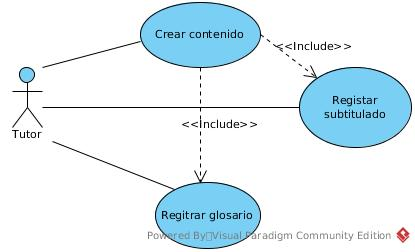
\includegraphics[scale=0.7]{useCaseTranslation}
	}
	\captionof{figure}{Diagrama de caso de uso para glosario y subtitulado}
	\source{fuente: (Elaboración propia)}
	\label{fig:Diagrama de caso de uso para glosario y subtitulado}
\end{minipage}

En la figura \ref{fig:Diagrama de clases para glosario y subtitulado},
el diagrama de clases representa la abstracción de datos y comunicación
de clases.

\begin{minipage}{1.0\textwidth}
	\centering
	\fbox{
		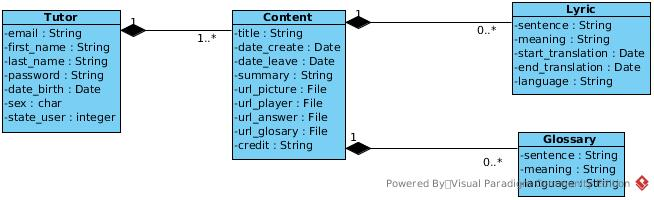
\includegraphics[scale=0.7]{classTranslation}
	}
	\captionof{figure}{Diagrama de clases para glosario y subtitulado}
	\source{fuente: (Elaboración propia)}
	\label{fig:Diagrama de clases para glosario y subtitulado}
\end{minipage}

En la figura \ref{fig:Diagrama de secuencia para glosario y subtitulado},
el diagrama de secuencia representa la comunicación de un rol autorregulado
y las clases de glosario y subtitulado.

\begin{minipage}{1.0\textwidth}
	\centering
	\fbox{
		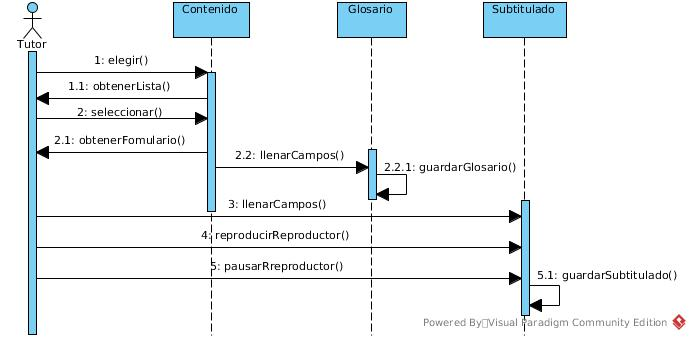
\includegraphics[scale=0.6]{sequenceTranslation}
	}
	\captionof{figure}{Diagrama de secuencia para glosario y subtitulado}
	\source{fuente: (Elaboración propia)}
	\label{fig:Diagrama de secuencia para glosario y subtitulado}
\end{minipage}

\subsection{Modelo de componente}

En la figura \ref{fig:Modelo de datos para glosario y subtitulado}, el modelo
de datos representa la persistencia de glosario y subtitulado.

\begin{minipage}{1.0\textwidth}
	\centering
	\fbox{
		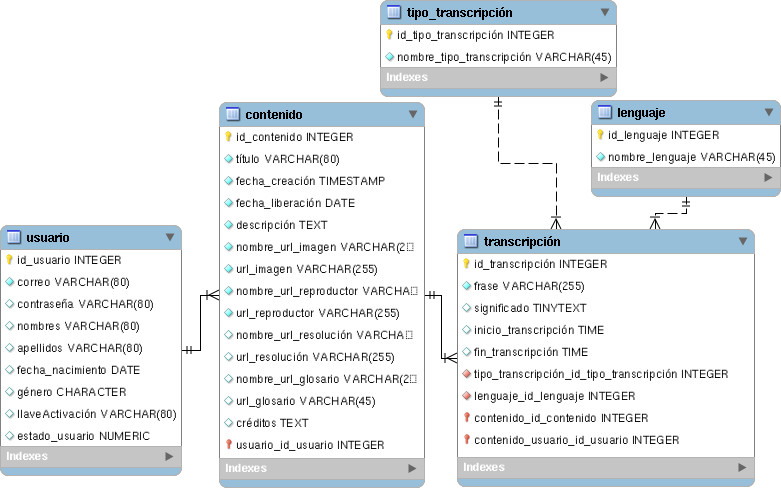
\includegraphics[scale=0.6]{modelTranslation}
	}
	\captionof{figure}{Modelo de datos para glosario y subtitulado}
	\source{fuente: (Elaboración propia)}
	\label{fig:Modelo de datos para glosario y subtitulado}
\end{minipage}

\subsection{Componente}

\begin{itemize}

\item \textbf{Glosario de sentencia}, permite crear una frase con respectivo
significado.
\item \textbf{Subtitulado de transcripción}, permite relacionar reproductor
de tipo audio con transcripción.

\end{itemize}

\textbf{Glosario} en la figura \ref{fig:Formulario de registro para glosario}, el
formulario brinda la funcionalidad de crear glosario; considerando lo
siguientes campos de tipo, frase, lenguaje destino y significado.

\begin{minipage}{1.0\textwidth}
	\centering
	\fbox{
		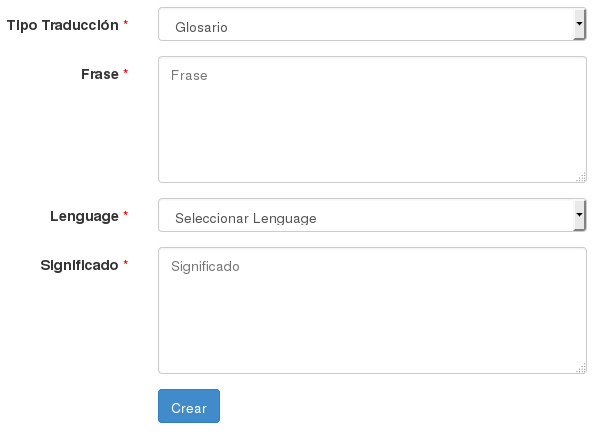
\includegraphics[scale=0.6]{formGlossary}
	}
	\captionof{figure}{Formulario de registro para glosario}
	\source{fuente: (Elaboración propia)}
	\label{fig:Formulario de registro para glosario}
\end{minipage}

\textbf{Subtitulado} en la figura \ref{fig:Formulario de registro para subtitulado},
el formulario permite la creación de un subtitulado conformado de frase, lenguaje
destino, significado, reproductor, tiempo inicio y tiempo fin.

\begin{minipage}{1.0\textwidth}
	\centering
	\fbox{
		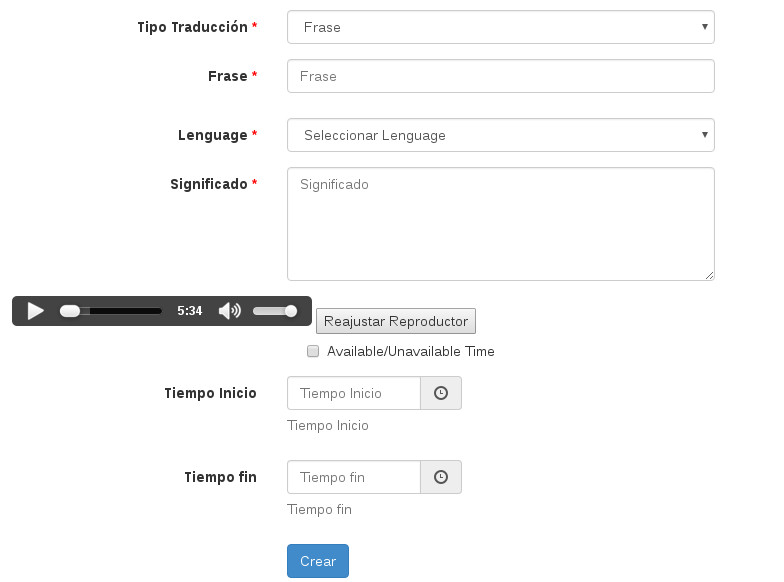
\includegraphics[scale=0.6]{formLyric}
	}
	\captionof{figure}{Formulario de registro para subtitulado}
	\source{fuente: (Elaboración propia)}
	\label{fig:Formulario de registro para subtitulado}
\end{minipage}

En la figura \ref{fig:Diagrama de estado para subtitulado}, el diagrama de
esto representa los diferentes estados que tiene un reproductor para la
definición de los tiempos de un subtitulado. 

\begin{minipage}{1.0\textwidth}
	\centering
	\fbox{
		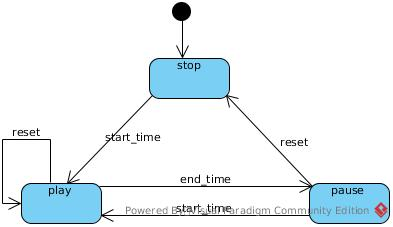
\includegraphics[scale=0.7]{stateLyric}
	}
	\captionof{figure}{Diagrama de estado para subtitulado}
	\source{fuente: (Elaboración propia)}
	\label{fig:Diagrama de estado para subtitulado}
\end{minipage}

\subsection{Implementar componente}

\begin{itemize}

\item \textbf{Subtitulado - implementar en el cliente} el segmento de código
obtiene dos listas de transcripción origen y traducción destino.

\begin{lstlisting}[caption={Llenado de elemento en subtitulado.}, label={lst:fillSubtitle}]
var myPlayer = document.getElementById("audio-player"); // get object audio player
var flag = false; // flag for run one time
myPlayer.addEventListener("play", function () { // add event play listener
if (!flag) { // verify no change flag
    $.ajax({ // get property through ajax
        type: "POST",
        url: "<?php echo CController::createUrl('Translation/getItemSentences');
        ?>",
        data: {
            idTypeTranslation: "<?php echo Yii::app()->params[
                'idTypeTranslationSentence']; ?>",
            idContent: "<?php echo Yii::app()->getRequest()->getParam(
                    'id_content'); ?>",
            idUser: "<?php echo Yii::app()->getRequest()->getParam(
                    'user_id_user'); ?>",
            idLanguage: "<?php echo $model_translation->language_id_language; ?>"
    },
    dataType: "html",
    success: function (data) {
    var div = document.getElementById("idSentence");
    div.innerHTML = data;
    }
    });
    .....
    flag = true; // change flag
    play(myPlayer); // call function for show subtitle
}
}, false);
\end{lstlisting}

\item \textbf{Subtitulado - implementar en el cliente} el segmento de código
realiza la acción necesaria para mostrar/ocultar el subtitulado de podcast,
por lo cual el botón realizar el evento de control.

\begin{lstlisting}[caption={Control de mostrar/ocultar subtitulado.}]
function play(myPlayer) {
    var controlDuplicate = [];
    myPlayer.ontimeupdate = function () {
    var currentTimePhrase = myPlayer.currentTime; // get currentTime player
    var currentIDStart = ""; // identifier for start_translation, end_translation
    var currentIDEnd = "";
    var timeConvert = ""; // time converter min:seg
    var hr = Math.floor(currentTimePhrase / 3600); //convert from seg to min
    var min = Math.floor((currentTimePhrase - (hr * 3600)) / 60);
    var sec = Math.floor(currentTimePhrase - (hr * 3600) - (min * 60));
    if (min < 10) { // if min is less 10 add 0
        min = "0" + min;
    }
    if (sec < 10) { // if sec is less 10 add 0
        sec = "0" + sec;
    }
    timeConvert = min + ':' + sec + ':00';
    if (controlDuplicate.length == 0) {
        controlDuplicate.push(timeConvert);
    $('#idSentence li').filter(':not([start_time_translation]),
        [start_time_translation="' + timeConvert + '"]').addClass(
        'sentence_show');
    ...
    } else if (controlDuplicate[controlDuplicate.length - 1] != timeConvert) {
        controlDuplicate.push(timeConvert);
    $('#idSentence li').filter(':not([start_time_translation]),
        [start_time_translation="'+ timeConvert + '"]').addClass(
        'sentence_show');
    $('#idSentence li').filter(':not([start_time_translation]),
        [end_time_translation="' + timeConvert + '"]').removeClass(
        'sentence_show');
    ...
    }
    };
}
\end{lstlisting}

\end{itemize}

\subsection{Problema/Solución de componente}

\begin{itemize}

\item \textbf{Glosario de término}

\begin{itemize}

\item Uso de registro de un solo formulario para la definición de glosario y
subtitulado.

\end{itemize}

\begin{enumerate}

\item \textbf{Validación de campos en formulario} en el segmento de código
la validación de un escenario para glosario se definido en el modelo de clase.

\begin{lstlisting}[language=PHP, caption={Validación de campos para escenario glosario.}]
public function actionCreate($id_content, $id_user) {
...
if (isset($_POST['Translation'])) {
    $model->attributes = $_POST['Translation'];
    $model->content_id_content = $id_content; // fill property
    $model->content_user_id_user = $id_user;
    if ($_POST['Translation']['type_translation_id_type_translation'] == 
            Yii::app()->params['idTypeTranslationSentence']) {
        $model->setScenario('sentence'); //change scenary
        $model->start_translation = $_POST['Translation']['start_translation'];
        $model->end_translation = $_POST['Translation']['end_translation'];
    } elseif ($_POST['Translation']['type_translation_id_type_translation'] == 
            Yii::app()->params['idTypeTranslationDictionary']) {
        $model->setScenario('dictionary'); //change scenary
    }
    if ($model->validate()) {
        $this->saveModel($model);
        ...
    }
}
...
}
}
\end{lstlisting}

\end{enumerate}

\item \textbf{Subtitulado de reproductor}

\begin{itemize}

\item Definición de formato de hora de minutos para tiempo inicio y
minuto tiempo final.
\item Frase de transcripción de tiempo inicio y tiempo final.

\end{itemize}

\begin{enumerate}

\item \textbf{Formato de hora} el reproductor define el valor a través de
la acción reproducir/detener, de manera que el tiempo debe considerar el
siguiente formato de mm:ss

Por tanto la unidad de tiempo obtenida de un reproductor es insuficiente para
esto agregar un cero por delante.

\begin{lstlisting}[caption={Generador de formato para minuto y segundo.}]
var myPlayer = document.getElementById("playerMyTranslation");
myPlayer.addEventListener("play", function () {
    var status_start_translation = document.getElementById(
        'start_translation').disabled;
    if (!status_start_translation) {
        var second_start_translation = Math.floor(myPlayer.
            currentTime % 60);
        if (second_start_translation < 10) {
            second_start_translation = "0" + 
            second_start_translation;
        }
        var minute_start_translation = Math.floor((myPlayer.currentTime / 60)
                % 60);
        if (minute_start_translation < 10) {
            minute_start_translation = "0" + 
            minute_start_translation;
        }
        document.getElementById('start_translation').value = 
                minute_start_translation +':' + second_start_translation;
        }
}, false);
...
\end{lstlisting}

\item \textbf{Revertir valor de inicio} el usuario con rol tutor puede
realizar una equivocación al momento definir el evento del reproductor,
para esto se recomienda revertir con el siguiente segmento de código.

\begin{lstlisting}[caption={Revertir valor de tiempo y reproductor.}]
function resetPlayer() {
    var status_start_translation = document.getElementById(
        'start_translation').disabled;
    var status_end_translation = document.getElementById(
        'end_translation').disabled;
    var myPlayer = document.getElementById("playerMyTranslation");
    if (!status_start_translation && !status_end_translation) {
        if (myPlayer.play) {
        myPlayer.currentTime = 0;
        document.getElementById('start_translation').value = 0; // set start
        document.getElementById('end_translation').value = 0; // set end
        }
    }
}
\end{lstlisting}

\end{enumerate}

\end{itemize}

\section{\textquestiondown Cómo representar glosario y subtitulado?}

Se agrega contenido semántico a: glosario y subtitulado. 

\subsection{Componente}

\begin{itemize}

\item \textbf{Representación de glosario uso de h-entry}
el esquema de representación de un micro-formato de tipo h-entry para la
representación de un glosario de podcast. \cite{hEntry}

\begin{itemize}

\item \textbf{p-name} nombre entrada/título.
\item \textbf{p-summary} breve resumen entrada.
\item \textbf{e-content} contenido completo entrada.
\item \textbf{dt-published} cuando se publicó la entrada.
\item \textbf{dt-updated} cuando se actualiza la entrada.
\item \textbf{p-author} que escribió la entrada, opcional mente incorporados
h-card.
\item \textbf{p-category} categoría entrada tags.
\item \textbf{u-url} URL del enlace permanente entrada.
\item \textbf{u-uid} identificador único universal, la entrada URL canónica
normalmente.
\item \textbf{p-location} la ubicación de la entrada fue publicada a partir,
opcional mente embed h-card, or h-geo.
\item \textbf{u-syndication} URL de copias sindicatos de este post, La propiedad
equivalente de rel-syndication.
\item \textbf{u-in-reply-to} la URL cual h-entry se considera respuesta a, 
opcional mente una h-cite.

\end{itemize}

En la figura \ref{fig:Presentación glosario}, el glosario podcast tiene como
elementos de frase y significado. 

\begin{minipage}{1.0\textwidth}
	\centering
	\fbox{
		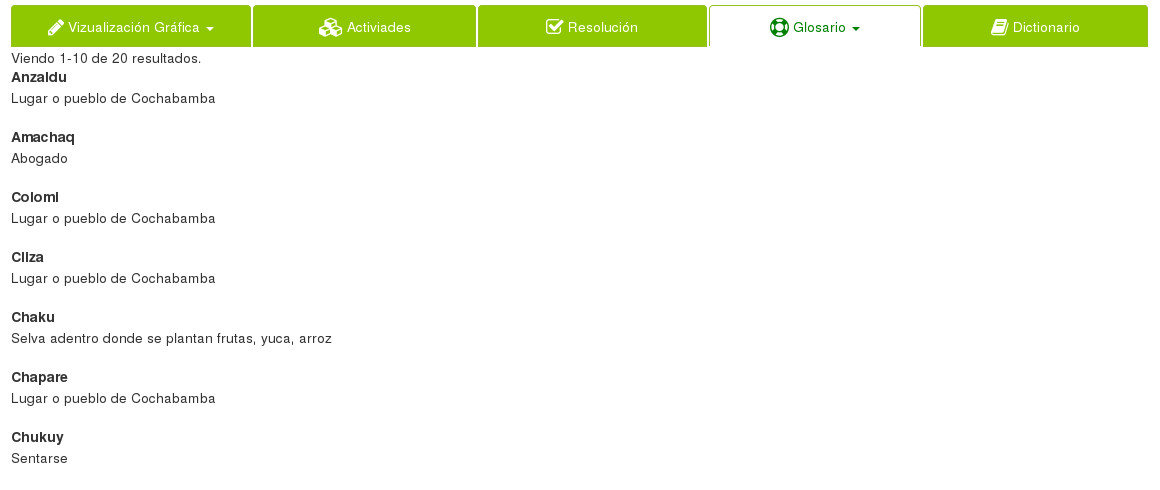
\includegraphics[scale=0.5]{glossary}
	}
	\captionof{figure}{Presentación glosario}
	\source{fuente: (Elaboración propia)}
	\label{fig:Presentación glosario}
\end{minipage}

\item \textbf{Representación de subtitulado} microformato tiene una
cantidad definida de tipos, se debe utilizar microformato 2 considerado
como extension de funcionalidad. 

\textbf{microformato 2}

\begin{itemize}

\item 'h-*' de nombres de clase raíz.
\item 'p-*' para las características simples (texto).
\item 'u-*' para las características URL.
\item 'dt-*' para la características de fecha/hora.
\item 'e-*' para las propiedades de marcado incrustado. \cite{microformats2}
 
\end{itemize}

Se propone la siguiente estructura para agregar contenido semántico para un
subtitulado.

\begin{enumerate}

\item \textbf{h-x-lyrics} raíz de esquema.

	\begin{enumerate}
	
		\item \textbf{p-lyric h-x-lyric} contenedora de elementos.
		
			\begin{enumerate}

				\item \textbf{p-start-time} representa tiempo inicio.
				\item \textbf{p-content} representa contenido.
				\item \textbf{p-end-time} representa tiempo fin.			

				\end{enumerate}					

	\end{enumerate}

\end{enumerate}

En la figura \ref{fig:Representación de subtitulado}, el reproductor de audio
sincroniza con subtitulado.

\begin{minipage}{1.0\textwidth}
	\centering
	\fbox{
		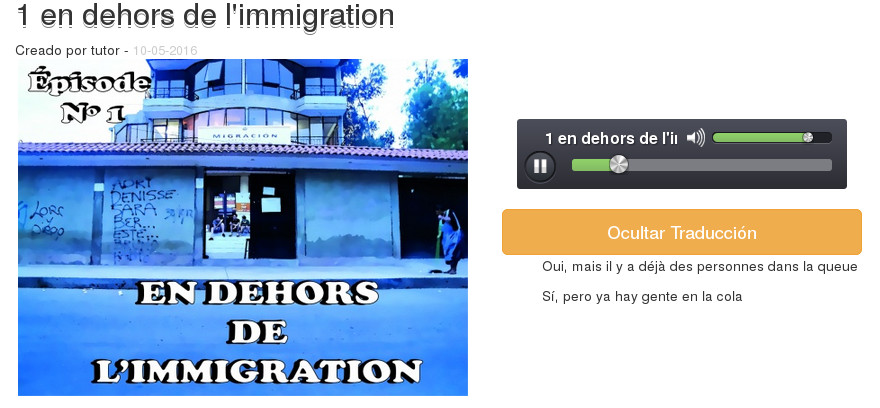
\includegraphics[scale=0.6]{lyric}
	}
	\captionof{figure}{Representación de subtitulado}
	\source{fuente: (Elaboración propia)}
	\label{fig:Representación de subtitulado}
\end{minipage}

\end{itemize}

\subsection{Implementar componente}

\begin{itemize}

\item \textbf{Glosario - implementar en el cliente} el segmento de código
agrega contenido semántico para glosario tiene un microformato de tipo
h-entry.

\begin{lstlisting}[language = PHP, caption={Representación de glosario.}]
<dl class="h-entry">
    <dt class="p-name">
        <?php echo $data->sentence; ?> 
    </dt> 
    <dd class="p-content">
        <?php echo $data->meaning; ?> 
    </dd>
</dl>
\end{lstlisting}

\item \textbf{Subtitulado - implementar en el cliente} el segmento de código
describe la agregación de la estructura propuesta para subtitulado.

\begin{lstlisting}[language = PHP, caption={Estructura de sentencia.}]
<ul class="h-sentence-lyrics ul_hide">
    <?php foreach ($model_translations as $translation): ?>  
    <li class="p-lyric h-sentence-lyric"> 
        <time class="p-start-time"> <?php echo $translation->start_translation;
        ?> </time>    
        <span class="p-content" > <?php echo $translation->sentence; ?></span>
        <time class="p-end-time"> <?php echo $translation->end_translation;?> 
           </time>
    </li>
    <?php endforeach; ?>
</ul>
...
\end{lstlisting}

\end{itemize}

\subsection{Problema/Solución de componente}

\begin{itemize}

\item \textbf{Representación de glosario}

\begin{itemize}

\item Uso de HTML5 \footnote{HTML5: Es una versión del lenguaje de marcado
de hipertexto, el lenguaje de programación estándar para describir el
contenido y la apariencia de las páginas web. \cite{html5}}  para agregar 
contenido semántico.

\begin{enumerate}

\item \textbf{Uso de estándar HTML5} el uso de documento HTML5 permite el
uso estándar para microformato.

\end{enumerate}

\end{itemize}

\item \textbf{Representación de subtitulado}

\begin{itemize}

\item Agregación de microformato en el lado del servidor.

\end{itemize}

\begin{enumerate}
 
\item \textbf{Llenado en el lado del servidor} el proceso de subtitulado
tiene que ser en el lado del servidor, un extractor externo de microformato
realiza comunicación por medio de una solicitud vía servidor.

\begin{lstlisting}[language = PHP, caption={Acción de obtención y envió para vista podcast.}]
public function actionViewContent($id_content, $user_id_user, 
        $type_content_id_type_content, $category_id_category) {
    Yii::app()->theme = 'front';
    $model = $this->loadModel($id_content, $user_id_user, 
            $type_content_id_type_content, $category_id_category);
    $model_user = new User('registerSuscribe'); // new model User
    $model_user->category_id = $category_id_category;
    $model_translate = Translate::getTranslate($id_content);
    $model_translation = Translation::model()->findByAttributes(array(
        'content_id_content' => $id_content, 'content_user_id_user' => 
        $user_id_user)); // get property model
    $model_translations = Translation::model()->findAllByAttributes(array(
        'type_translation_id_type_translation' => $type_content_id_type_content,
        'content_id_content' => $id_content, 'content_user_id_user' => 
        $user_id_user), array('order' => 'start_translation asc'));
    if (!Yii::app()->user->isGuest){ // is Login
        $model_detail_subscriptions = DetailSubscription::model()->
            findAllByAttributes(array('subscription_user_id_user' => 
                Yii::app()->user->id));
    }else{
        $model_detail_subscriptions = array();
    }
    $this->render('viewContent', array('model' => $model, 'model_user' => 
        $model_user, 'model_detail_subscriptions' => $model_detail_subscriptions, 
        'model_translate' => $model_translate, 'model_translation' => 
        $model_translation, 'model_translations' => $model_translations));
    }
}
\end{lstlisting}

\end{enumerate}

\end{itemize}

\section{\textquestiondown Cómo realizar pruebas unitaria de suscriptor, integración de audio y vídeo?}

Uso de prueba unitaria sobre la capa modelo.

Además, las pruebas de integración requiere el uso de un servidor web autónomo. 

\subsection{Componente}

\begin{itemize}

\item \textbf{Prueba unitaria de suscripción} en la figura 
\ref{fig:Diagrama de clase representa dependencia de suscripción}
el diagrama de clases representa la dependencia para el proceso de prueba
unitaria \footnote{prueba: La prueba de software es un método de evaluación
de la funcionalidad de un programa de software. \cite{test}}.

\begin{minipage}{1.0\textwidth}
	\centering
	\fbox{
		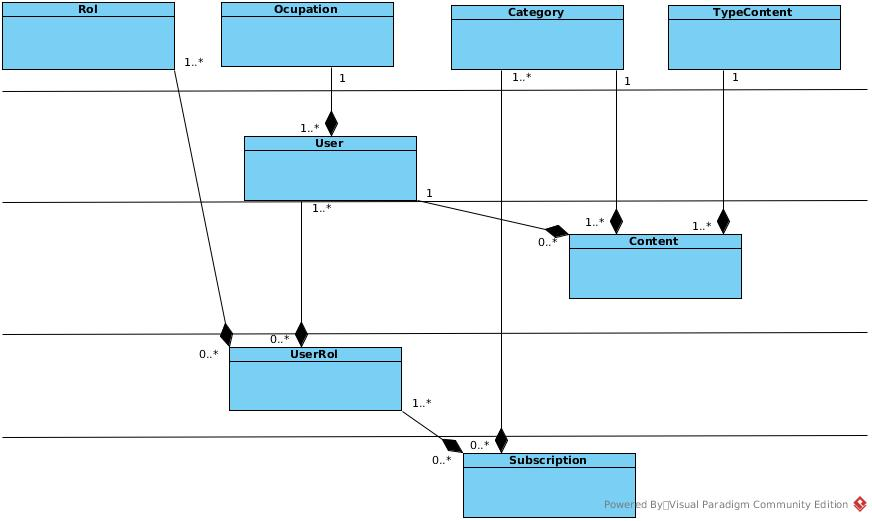
\includegraphics[scale=0.5]{subscriptionTest}
	}
	\captionof{figure}{Diagrama de clase representa dependencia de suscripción}
	\source{fuente: (Elaboración propia)}
	\label{fig:Diagrama de clase representa dependencia de suscripción}
\end{minipage}

\end{itemize}

\subsection{Reporte de prueba}

\begin{itemize}

\item \textbf{Prueba unitaria de suscripción} únicamente, esta sección utiliza
el uso de reporte para especificar la ejecución.

Acorde con clase suscripción subsección \ref{serviceFeed}, se realiza la
prueba necesaria.

% report test 1
\begin{minipage}[!htb]{\hsize}\centering
\begin{tabular}{|c|c|}
\hline
\multicolumn{2}{|c|}{\textbf{Caso Prueba de Unidad}} \\ \hline
\multicolumn{1}{|l|}{Caso de prueba ID: 1} & \multicolumn{1}{l|}{Nombre de módulo: Categoría} \\ \hline
\multicolumn{1}{|l|}{Título prueba: executeOneLevelCategory} & \multicolumn{1}{l|}{Ejecución de prueba: 20-06-2016} \\ \hline
\multicolumn{1}{|l|}{Prioridad de prueba: Alto} & \multicolumn{1}{l|}{Fecha diseño de prueba: 11-02-2016} \\ \hline
\multicolumn{2}{|l|}{Pre-condición: BD vacía.} \\ \hline
\multicolumn{2}{|l|}{Dependencia: Categoría nivel zero.} \\ \hline
\textbf{Pasos de prueba} & \textbf{Datos de prueba} \\ \hline
\begin{tabular}[c]{@{}c@{}}Registrar categoría\\ de un nivel uno.\end{tabular} & \multicolumn{1}{l|}{\begin{tabular}[c]{@{}l@{}}nombre\_categoría='Quechua Psicosocial' \\ nombre\_url\_imagen\_categoría='psicosocial.jpg' \\ url\_imagen\_categoría='123\_psicosocial.jpg' \\ descripción\_categoría='descripción psicosocial' \\ descripción\_creditos='descripción creditos' \\ descripción\_objetivo='descripción objetivo' \\ categoría\_id\_categoría=6\end{tabular}} \\ \hline
\textbf{Resultado esperado} & \textbf{Resultado actual} \\ \hline
verdad & verdad \\ \hline
\textbf{Estado} & \textbf{Notas} \\ \hline
éxito & nombre categoría debe ser único. \\ \hline
\end{tabular}
\captionof{table}{Reporte prueba 1}
\source{fuente: (Elaboración propia)}
\label{Reporte prueba 1}
\end{minipage}

%report test 2
\begin{minipage}[!htb]{\hsize}\centering
\begin{tabular}{|c|c|}
\hline
\multicolumn{2}{|c|}{\textbf{Caso Prueba de Unidad}} \\ \hline
\multicolumn{1}{|l|}{Caso de prueba ID: 2} & \multicolumn{1}{l|}{Nombre de módulo: Ocupación} \\ \hline
\multicolumn{1}{|l|}{Título prueba: executeOcupation} & \multicolumn{1}{l|}{Ejecución de prueba: 20-06-2016} \\ \hline
\multicolumn{1}{|l|}{Prioridad de prueba: Alto} & \multicolumn{1}{l|}{Fecha diseño de prueba: 11-02-2016} \\ \hline
\multicolumn{2}{|l|}{Pre-condición: BD vacía.} \\ \hline
\multicolumn{2}{|l|}{Dependencia: Ocupación nivel zero.} \\ \hline
\textbf{Pasos de prueba} & \textbf{Datos de prueba} \\ \hline
\begin{tabular}[c]{@{}c@{}}Registrar ocupación \\ de un nivel uno.\end{tabular} & \multicolumn{1}{l|}{\begin{tabular}[c]{@{}l@{}}nombre\_ocupación='Gerente de serivicos administrativos' \\ ocupación\_id\_ocupación=76\end{tabular}} \\ \hline
\textbf{Resultado esperado} & \textbf{Resultado actual} \\ \hline
verdad & verdad \\ \hline
\textbf{Estado} & \textbf{Notas} \\ \hline
éxito & nombre ocupación debe ser único. \\ \hline
\end{tabular}
\captionof{table}{Reporte prueba 2}
\source{fuente: (Elaboración propia)}
\label{Reporte prueba 2}
\end{minipage}

% report test 3
\begin{minipage}[!htb]{\hsize}\centering
\begin{tabular}{|c|c|}
\hline
\multicolumn{2}{|c|}{\textbf{Caso Prueba de Unidad}} \\ \hline
\multicolumn{1}{|l|}{Caso de prueba ID: 3} & \multicolumn{1}{l|}{Nombre de módulo: Rol} \\ \hline
\multicolumn{1}{|l|}{Título prueba: executeRol} & \multicolumn{1}{l|}{Ejecución de prueba: 20-06-2016} \\ \hline
\multicolumn{1}{|l|}{Prioridad de prueba: Alto} & \multicolumn{1}{l|}{Fecha diseño de prueba: 12-02-2016} \\ \hline
\multicolumn{2}{|l|}{Pre-condición: BD vacía.} \\ \hline
\multicolumn{2}{|l|}{Dependencia:} \\ \hline
\textbf{Pasos de prueba} & \textbf{Datos de prueba} \\ \hline
Registrar nombre rol. & \multicolumn{1}{l|}{nombre\_rol='autorregulado'} \\ \hline
\textbf{Resultado esperado} & \textbf{Resultado actual} \\ \hline
verdad & verdad \\ \hline
\textbf{Estado} & \textbf{Notas} \\ \hline
éxito & nombre rol debe ser único. \\ \hline
\end{tabular}
\captionof{table}{Reporte prueba 3}
\source{fuente: (Elaboración propia)}
\label{Reporte prueba 3}
\end{minipage}

% report test 4
\begin{minipage}[!htb]{\hsize}\centering
\begin{tabular}{|c|c|}
\hline
\multicolumn{2}{|c|}{\textbf{Caso Prueba de Unidad}} \\ \hline
\multicolumn{1}{|l|}{Caso de prueba ID: 4} & \multicolumn{1}{l|}{Nombre de módulo: Usuario} \\ \hline
\multicolumn{1}{|l|}{Título prueba: executeUserOneLevelOcupation} & \multicolumn{1}{l|}{Ejecución de prueba: 20-06-2016} \\ \hline
\multicolumn{1}{|l|}{Prioridad de prueba: Alto} & \multicolumn{1}{l|}{Fecha diseño de prueba: 18-02-2016} \\ \hline
\multicolumn{2}{|l|}{Pre-condición: Usuario disponible.} \\ \hline
\multicolumn{2}{|l|}{Dependencia: Ocupación.} \\ \hline
\textbf{Pasos de prueba} & \textbf{Datos de prueba} \\ \hline
Registrar datos de usuario. & \multicolumn{1}{l|}{\begin{tabular}[c]{@{}l@{}}correo='juan@gmail.com' \\ nombre\_usuario='omarhuanca' \\ contraseña='123' \\ estado\_usuario=1 \\ llaveActivación='1a2b3c' \\ ocupación\_id\_ocupación=84\end{tabular}} \\ \hline
\textbf{Resultado esperado} & \textbf{Resultado actual} \\ \hline
verdad & verdad \\ \hline
\textbf{Estado} & \textbf{Notas} \\ \hline
éxito & \begin{tabular}[c]{@{}c@{}}nombre\_usuario, correo \\ debe ser único.\end{tabular} \\ \hline
\end{tabular}
\captionof{table}{Reporte prueba 4}
\source{fuente: (Elaboración propia)}
\label{Reporte prueba 4}
\end{minipage}

% report test 5
\begin{minipage}[!htb]{\hsize}\centering
\begin{tabular}{|c|c|}
\hline
\multicolumn{2}{|c|}{\textbf{Caso Prueba de Unidad}} \\ \hline
\multicolumn{1}{|l|}{Caso de prueba ID: 5} & \multicolumn{1}{l|}{Nombre de módulo: Contenido} \\ \hline
\multicolumn{1}{|l|}{Título prueba: executeContentTypeAudio} & \multicolumn{1}{l|}{Ejecución de prueba: 20-06-2016} \\ \hline
\multicolumn{1}{|l|}{Prioridad de prueba: Medio} & \multicolumn{1}{l|}{Fecha diseño de prueba: 18-02-2016} \\ \hline
\multicolumn{2}{|l|}{Pre-condición: Usuario disponible, Contenido disponible.} \\ \hline
\multicolumn{2}{|l|}{Dependencia: Ocupación, Usuario, Categoría, TipoContenido.} \\ \hline
\textbf{Pasos de prueba} & \textbf{Datos de prueba} \\ \hline
Registrar datos de contenido. & \multicolumn{1}{l|}{\begin{tabular}[c]{@{}l@{}}título='Contenido 1' \\ fecha\_creación='2016-06-20 12:10:00' \\ fecha\_liberación='2016-06-21' \\ descripción='descripción' \\ nombre\_url\_imagen='imagen contenido 1' \\ url\_imagen='123\_imagen\_contenido\_1' \\ nombre\_url\_reproductor='reproductor contenido 1' \\ url\_reproductor='456\_reproductor\_1' \\ nombre\_url\_respuesta='documento respuesta 1' \\ url\_respuesta=789\_documento\_respuesta\_1' \\ nombre\_url\_glosario='documento glosario 1' \\ url\_glosario='1011\_documento\_glosario\_1' \\ créditos='créditos contenido 1' \\ contenido\_estado=1 \\ tipo\_contenido\_id\_tipo\_contenido=1 \\ categoría\_id\_categoría=28\end{tabular}} \\ \hline
\textbf{Resultado esperado} & \textbf{Resultado actual} \\ \hline
verdad & verdad \\ \hline
\textbf{Estado} & \textbf{Notas} \\ \hline
éxito & \begin{tabular}[c]{@{}c@{}}fecha liberación debe \\ ser mayora fecha de creación.\end{tabular} \\ \hline
\end{tabular}
\captionof{table}{Reporte prueba 5}
\source{fuente: (Elaboración propia)}
\label{Reporte prueba 5}
\end{minipage}

% report test 6
\begin{minipage}[!htb]{\hsize}\centering
\begin{tabular}{|c|c|}
\hline
\multicolumn{2}{|c|}{\textbf{Caso Prueba de Unidad}} \\ \hline
\multicolumn{1}{|l|}{Caso de prueba ID: 6} & \multicolumn{1}{l|}{Nombre de módulo: UsuarioRol} \\ \hline
\multicolumn{1}{|l|}{Título prueba: executeUserRol} & \multicolumn{1}{l|}{Ejecución de prueba: 20-06-2016} \\ \hline
\multicolumn{1}{|l|}{Prioridad de prueba: Medio} & \multicolumn{1}{l|}{Fecha diseño de prueba: 18-02-2016} \\ \hline
\multicolumn{2}{|l|}{Pre-condición: Usuario disponible.} \\ \hline
\multicolumn{2}{|l|}{Dependencia: Ocupación, Usuario, Rol.} \\ \hline
\textbf{Pasos de prueba} & \textbf{Datos de prueba} \\ \hline
Registrar datos de usuario\_rol. & \multicolumn{1}{l|}{\begin{tabular}[c]{@{}l@{}}usuario\_id\_usuario=35\\ rol\_id\_rol=7\end{tabular}} \\ \hline
\textbf{Resultado esperado} & \textbf{Resultado actual} \\ \hline
verdad & verdad \\ \hline
\textbf{Estado} & \textbf{Notas} \\ \hline
éxito &  \\ \hline
\end{tabular}
\captionof{table}{Reporte prueba 6}
\source{fuente: (Elaboración propia)}
\label{Reporte prueba 6}
\end{minipage}

% report test 7
\begin{minipage}[!htb]{\hsize}\centering
\begin{tabular}{|c|c|}
\hline
\multicolumn{2}{|c|}{\textbf{Caso Prueba de Unidad}} \\ \hline
\multicolumn{1}{|l|}{Caso de prueba ID: 7} & \multicolumn{1}{l|}{Nombre de módulo: Suscripción} \\ \hline
\multicolumn{1}{|l|}{Título prueba: executeSubscription} & \multicolumn{1}{l|}{Ejecución de prueba: 20-06-2016} \\ \hline
\multicolumn{1}{|l|}{Prioridad de prueba: Medio} & \multicolumn{1}{l|}{Fecha diseño de prueba: 18-02-2016} \\ \hline
\multicolumn{2}{|l|}{Pre-condición: Usuario disponible, Contenido disponible.} \\ \hline
\multicolumn{2}{|l|}{Dependencia: Ocupación, Usuario, Rol, UsuarioRol, Categoría.} \\ \hline
\textbf{Pasos de prueba} & \textbf{Datos de prueba} \\ \hline
Registrar datos de Suscripción. & \multicolumn{1}{l|}{\begin{tabular}[c]{@{}l@{}}categoría\_id\_categoría=7\\ id\_usuario\_rol=2\\ usuario\_id\_usuario=2\\ rol\_id\_rol=2\end{tabular}} \\ \hline
\textbf{Resultado esperado} & \textbf{Resultado actual} \\ \hline
verdad & verdad \\ \hline
\textbf{Estado} & \textbf{Notas} \\ \hline
éxito &  \\ \hline
\end{tabular}
\captionof{table}{Reporte prueba 7}
\source{fuente: (Elaboración propia)}
\label{Reporte prueba 7}
\end{minipage}

En la figura \ref{fig:Ejecución de prueba para registrar suscripción}, la prueba
ejecuta la verificación dependencias para crear una suscripción. 

\begin{minipage}{1.0\textwidth}
	\centering
	\fbox{
		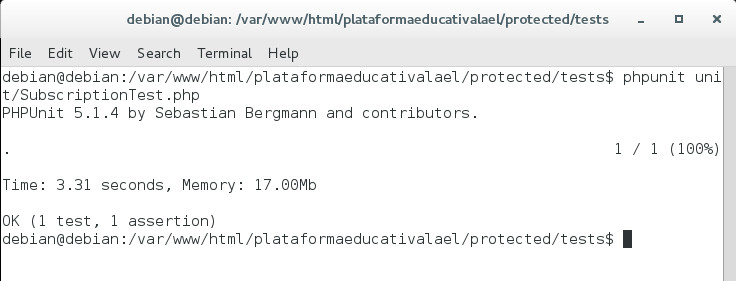
\includegraphics[scale=0.7]{runSubscriptionTest}
	}
	\captionof{figure}{Ejecución de prueba para registrar suscripción}
	\source{fuente: (Elaboración propia)}
	\label{fig:Ejecución de prueba para registrar suscripción}
\end{minipage}

\item \textbf{Prueba integración de audio y vídeo}

% report test 8
\begin{minipage}[!htb]{\hsize}\centering
\begin{tabular}{|c|c|}
\hline
\multicolumn{2}{|c|}{\textbf{Caso Prueba de Integración}} \\ \hline
\multicolumn{1}{|l|}{Caso de prueba ID: 8} & \multicolumn{1}{l|}{Nombre de módulo: Contenido} \\ \hline
\multicolumn{1}{|l|}{Título prueba: playAudioLocalHost} & \multicolumn{1}{l|}{Ejecución de prueba: 23-05-2016} \\ \hline
\multicolumn{1}{|l|}{Prioridad de prueba: Bajo} & \multicolumn{1}{l|}{Fecha diseño de prueba: 13-03-2016} \\ \hline
\multicolumn{2}{|l|}{Pre-condición: Contenido disponible, phpunit disponible, selenium webdriver ejecutado.} \\ \hline
\multicolumn{2}{|l|}{Dependencia: Ocupación, Usuario, Rol, UsuarioRol, Categoría, TipoContenido.} \\ \hline
\textbf{Pasos de prueba} & \textbf{Datos de prueba} \\ \hline
Obtener URL de podcast de tipo audio. & \multicolumn{1}{l|}{\begin{tabular}[c]{@{}l@{}}http://localhost/plataformaeducativalael/content/\\ viewContent?id\_content=1\&user\_id\_user=27\&\\ type\_content\_id\_type\_content=1\&\\ category\_id\_category=2\end{tabular}} \\ \hline
\textbf{Resultado esperado} & \textbf{Resultado actual} \\ \hline
verdad & verdad \\ \hline
\textbf{Estado} & \textbf{Notas} \\ \hline
éxito &  \\ \hline
\end{tabular}
\captionof{table}{Reporte prueba 8}
\source{fuente: (Elaboración propia)}
\label{Reporte prueba 8}
\end{minipage}

% report test 9
\begin{minipage}[!htb]{\hsize}\centering
\begin{tabular}{|c|c|}
\hline
\multicolumn{2}{|c|}{\textbf{Caso Prueba de Integración}} \\ \hline
\multicolumn{1}{|l|}{Caso de prueba ID: 9} & \multicolumn{1}{l|}{Nombre de módulo: Contenido} \\ \hline
\multicolumn{1}{|l|}{Título prueba: playVideoLocalHost} & \multicolumn{1}{l|}{Ejecución de prueba: 23-05-2016} \\ \hline
\multicolumn{1}{|l|}{Prioridad de prueba: Bajo} & \multicolumn{1}{l|}{Fecha diseño de prueba: 15-03-2016} \\ \hline
\multicolumn{2}{|l|}{Pre-condición: Contenido disponible, phpunit disponible, selenium webdriver ejecutado.} \\ \hline
\multicolumn{2}{|l|}{Dependencia: Ocupación, Usuario, Rol, UsuarioRol, Categoría, TipoContenido.} \\ \hline
\textbf{Pasos de prueba} & \textbf{Datos de prueba} \\ \hline
Obtener URL de podcast de tipo vídeo. & \multicolumn{1}{l|}{\begin{tabular}[c]{@{}l@{}}http://localhost/plataformaeducativalael/content/\\ viewContent?id\_content=2\&user\_id\_user=27\&\\ type\_content\_id\_type\_content=2\&\\ category\_id\_category=3\end{tabular}} \\ \hline
\textbf{Resultado esperado} & \textbf{Resultado actual} \\ \hline
verdad & verdad \\ \hline
\textbf{Estado} & \textbf{Notas} \\ \hline
éxito &  \\ \hline
\end{tabular}
\captionof{table}{Reporte prueba 9}
\source{fuente: (Elaboración propia)}
\label{Reporte prueba 9}
\end{minipage}

En la figura \ref{fig:Ejecución de prueba para reproducir audio y vídeo}, la prueba
ejecuta la prueba de integración de audio y vídeo. 

\begin{minipage}{1.0\textwidth}
	\centering
	\fbox{
		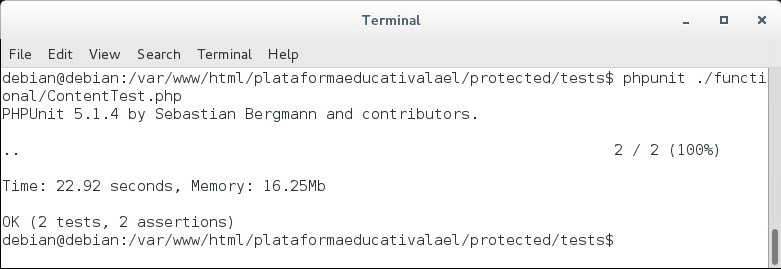
\includegraphics[scale=0.7]{runIntegrationTest}
	}
	\captionof{figure}{Ejecución de prueba para reproducir audio y vídeo}
	\source{fuente: (Elaboración propia)}
	\label{fig:Ejecución de prueba para reproducir audio y vídeo}
\end{minipage}


\end{itemize}

\subsection{Implementar componente}

\begin{itemize}

\item \textbf{Prueba unitaria} se hace uso de phpunit.

\item \textbf{Prueba de integración} se hace uso de selenium server
standalone y un módulo webdriver-bindings \footnote{webdriver-bindings:
Permite ejecutar pruebas funcionales utilizando funciones WebDriver de
selenium server 2.0 se ejecuta como plug-in de navegador remoto,
por lo que es mucho más fiable que la prueba estándar de selenium se inyecta
a través de JavaScript. \cite{webdriverTest}}.

\end{itemize}


\begin{itemize}

\item \textbf{Prueba unitaria}

\begin{enumerate}

\item \textbf{Implementar en el servidor} la definición de la prueba
\textquotedouble{executeSubscription} comprueba la ejecución de una
suscripción, la descripción de la prueba se la aprecia en 
cuadro \ref{Reporte prueba 7}.

\begin{lstlisting}[language=PHP, caption={Prueba de ejecución para suscripción.}]
class SubscriptionTest extends CDbTestCase {
    public function setUp() { // before each run test
        parent::setUp();
        ...
    }
    public function tearDown() { // after each run test
        parent::tearDown();
        ...
    }
    public function testCreateSubscription() {
        $subscription = new Subscription();     // create subscription
        $subscription->setAttributes(array(
        'category_id_category' => $this->categoryChild->id_category,
        'id_user_rol' => $this->userRol->id_user_rol,
        'user_id_user' => $this->userRol->user_id_user,
        'rol_id_rol' => $this->userRol->rol_id_rol
        ), false);
        $this->assertTrue($subscription->save(false));
    }
}
\end{lstlisting}

\item \textbf{Implementar en el servidor} la clase suscripción tiene una
función para control de excepción, se utilizó transacción \footnote{transacción:
Una secuencia de intercambio de información y el trabajo relacionado que se
trata como una unidad a efectos de satisfacer una solicitud como para
asegurar la integridad de la base de datos. \cite{transaction}} para manejo
de consistencia.

\begin{lstlisting}[language=PHP, caption={Función callback para control dependencia.}]
public function beforeSave() {
$res = false;
if ($this->isNewRecord) {
    $transaction = $this->dbConnection->beginTransaction(); // start transaction
    ...
    $category = Category::model()->findByAttributes(array('id_category' => 
        $this->category_id_category));
    if (isset($category)) {
        if (Yii::app()->params['idTypeContentAudio'] == 
                $this->type_content_id_type_content) {
            $user = User::model()->findByAttributes(array('id_user' => 
                $this->user_id_user, 'state_user' => Yii::app()->params[
                    'stateUserAvailable']));
            if (isset($user)) {
                $res = true;
            }
        }
    }
    if ($res) {
        $transaction->commit();
    } else {
        $transaction->rollback();
    }
    ...
} else {
    $res = true;
}
return $res;
}
\end{lstlisting}

\end{enumerate}

\item \textbf{Prueba de integración}

\begin{enumerate}

\item \textbf{Reproducir audio}

\begin{enumerate}

\item \textbf{Implementar en el servidor} la función de prueba
\textquotedouble{playAudioLocalHost} realiza la verificación de existencia
de un reproductor de tipo audio.

\begin{lstlisting}[language=PHP, caption={Prueba para reproducir reproductor de audio.}]
protected function setUp() {
    parent::setUp('localhost', 4444, 'firefox');
}
public function testPlayAudioLocalHost() {
    $this->get('http://localhost/plataformaeducativalael/content/'
    . 'viewContent/id_content/1/user_id_user/27/'
    . 'type_content_id_type_content/1/category_id_category/2');
    $this->click('audio-player');
    sleep(5);
    $elem = $this->findElementBy(LocatorStrategy::id,
        'audio-player');
    $this->assertNotNull($elem, 'Results not found!');
} 
\end{lstlisting}

\end{enumerate}

\item \textbf{Reproducir vídeo}

\begin{enumerate}

\item \textbf{Implementar en el servidor} la función de prueba
\textquotedouble{playVideoLocalHost} realiza la verificación de un reproductor
de tipo vídeo.

\begin{lstlisting}[language=PHP, caption={Prueba para reproducir reproductor de vídeo.}]
protected function setUp() {
    parent::setUp('localhost', 4444, 'firefox');
}
public function testPlayVideoLocalHost() {
    $this->get('http://localhost/plataformaeducativalael/content/'
    . 'viewContent?id_content=2&user_id_user=27&'
    . 'type_content_id_type_content=2&category_id_category=4');
    $this->click('audio-player');
    sleep(5);
    $elem = $this->findElementBy(LocatorStrategy::id,'audio-player');
    $this->assertNotNull($elem, 'Results not found!');
}
\end{lstlisting}

\end{enumerate}

\end{enumerate}

\end{itemize}

\subsection{Problema/Solución de componente}

\begin{itemize}

\item \textbf{Prueba unitaria}

\begin{itemize}

\item Instalar PHPUnit y dependencia desde composer.
\item Configurar archivos bootstrap y phpunit.xml sobre yii.
\item Editar archivos CWebTestCase para reconocimiento de sentencia phpunit.

\end{itemize}

\begin{enumerate}

\item \textbf{Uso dependencia phpunit} realizar la instalación de
dependencia para utilizar composer \footnote{composer: Es un gestor de
dependencias para PHP. Composer gestionará las dependencias que se requieren
en un proyecto por ejemplo. \cite{composer}}, a continuación se define la
ruta de instalación \textquotedouble{/project/protected/composer.json}

\begin{lstlisting}[caption={Dependencia de phpunit.}]
{
    "name": "kevin/protected",
    "authors": [
        {
            "name": "kevin",
            "email": "kevinflorenzdaus@gmail.com"
        }
    ],
    "require-dev": {
        "phpunit/phpunit": "3.7.*",
        "phpunit/phpunit-selenium": ">=1.2",
        "phpunit/dbunit": ">=1.2",
        "phpunit/phpunit-story": "*"
    }
}
\end{lstlisting}

\item \textbf{Configurar archivos bootstrap y phpunit}

Según \cite{testing} estos archivos son particulares, es como el guión de
entrada y es el punto de partida cuando se ejecuta una serie de pruebas.

\begin{lstlisting}[language=PHP, caption={Estructura de configuración de archivo bootstrap.}]
$vendors=dirname(__FILE__).'/../vendor/autoload.php';
$yiit=dirname(__FILE__).'/../../framework/yiit.php';
$config=dirname(__FILE__).'/../config/test.php'; //change the paths if necessary
require_once($vendors); // required file
require_once($yiit);
require_once(dirname(__FILE__).'/WebTestCase.php');
Yii::createWebApplication($config); // config app
\end{lstlisting}

En el segmento de código se representa la configuración de un archivo phpunit.xml
para uso de un navegador en específico.

\begin{lstlisting}[caption={Estructura de configuración archivo phpunit}]
<phpunit bootstrap="bootstrap.php"
	colors="false"
    convertErrorsToExceptions="true"
    convertNoticesToExceptions="true"
    convertWarningsToExceptions="true"
  	stopOnFailure="false">
<selenium>
	<browser name="Google Chrome" browser="*chrome" />
    <browser name="Firefox" browser="*firefox" />
</selenium>
</phpunit>
\end{lstlisting}

\item \textbf{Editar archivo CWebTestCase} el segmento de código muestra
el archivo CWebTestCase.php contempla tiene la configuración de inicio.

\begin{lstlisting}[language=PHP, caption={Cabecera de archivo CWebTestCase}, label={lst:fileCWebTestCase}]
Yii::import('system.test.CTestCase');
require_once('PHPUnit/Extensions/SeleniumTestCase.php');
\end{lstlisting}

A continuación el segmento de código muestra el archivo CWebTestCase.php
contiene una modificación. 

\begin{lstlisting}[language=PHP, caption={Modificación de instrucción.}, label={lst:replaceCWebTestCase}]
require_once('../../protected/vendor/phpunit/phpunit-selenium/
	PHPUnit/Extensions/SeleniumTestCase.php');
\end{lstlisting}

Como resultado, pruebas sobre Yii 1.X se debe realizar el cambio de sentencia
definido en segmento de código \ref{lst:replaceCWebTestCase}, por segmento de
código \ref{lst:fileCWebTestCase}.

\end{enumerate}

\item \textbf{Prueba integración}

\begin{itemize}

\item Instalación de navegador firefox.
\item Ejecutar sesión en selenium-server-standalone-Z.jar.
\item Inicio sesión en navegador chrome. 
 
\end{itemize}

\begin{enumerate}

\item \textbf{Instalación de navegador firefox} debian 8 utiliza un navegador
iceweasel reemplazar el por mozilla firefox.

\begin{lstlisting}[language=bash, caption={Instrucciones de instalación para mozilla firefox.}]
$ wget ftp://ftp.mozilla.org/pub/mozilla.org/..../firefox-Y.0.tar.bz2
cd /home/hugh/
$ tar -xjvf firefox-Y.0.tar.bz2
$ sudo rm -rf /opt/firefox*
$ sudo mv firefox /opt/firefoxY.0
$ sudo ln -sf /opt/firefoxY.0/firefox /usr/bin/firefox
\end{lstlisting}

La instalación de firefox tiene que ser de forma manual, un servidor web
como selenium-server-standalone-Z.jar utiliza la configuración de los
navegadores de uso general.

\item \textbf{Iniciar sesión selenium server standalone} el segmento de código
siguiente realiza el inicio del servidor web emulado.

\begin{lstlisting}[language=bash, caption={Ejecución de servidor server standalone.}]
$ java -jar  selenium-server-standalone-Z.jar
\end{lstlisting}

En la figura \ref{fig:Ejecución de selenium server standalone} selenium server
standalone empieza a funcionar.

\begin{minipage}{1.0\textwidth}
	\centering
	\fbox{
		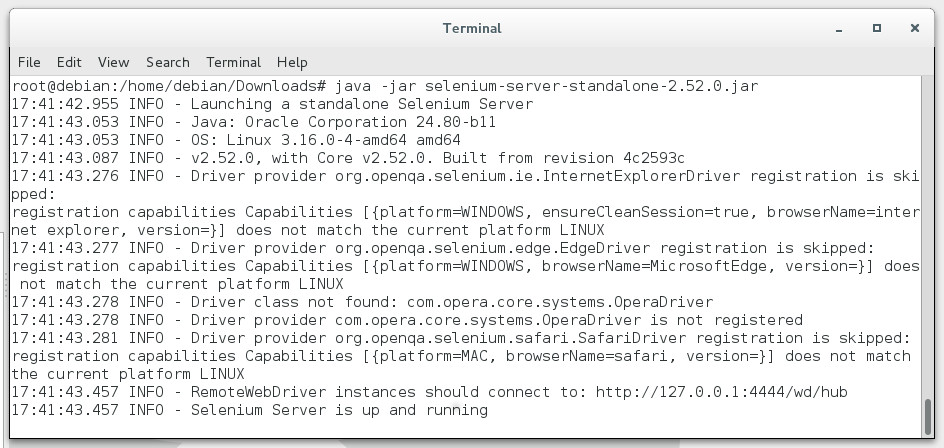
\includegraphics[scale=0.5]{executeSeleniumServer}
	}
	\captionof{figure}{Ejecución de selenium server standalone}
	\source{fuente: (Elaboración propia)}
	\label{fig:Ejecución de selenium server standalone}
\end{minipage}

Realizar una  prueba de integración requiere ejecutar
\textquotedouble{dirección local} 
\footnote{dirección local: http://127.0.0.1:4444/wd/hub}, sobre un
navegador firefox, seleccionar la opción y crear una sesión de trabajo.

\item \textbf{Inicio sesión navegador en chrome} selenium server standalone
tiene una configuración por defecto con firefox, si se desea utilizar otro
navegador como alternativa. En el segmento de código se realiza la
configuración por medio de un programa de control de chrome para ejecución
de selenium server standalone.

A continuación se ejecuta los siguientes coman-dos de descarga.

\begin{lstlisting}[language=bash, caption={Instalación de programa de control para chrome.}]
$ unzip /path/chromedriver_linux_64.zip
$ su root
# chmod +x chromedriver
\end{lstlisting}

De manera que se tiene que ejecutar el siguiente comando en el siguiente
segmento de código \textquotedouble{sobre una sola línea}.

\begin{lstlisting}[language=bash, caption={Configuración chromedriver en selenium server.}]
$ java -jar selenium-server-standalone-Z.jar -Dwebdriver.chrome.driver=
"/path/chromedriver"
\end{lstlisting}

A continuación en la figura \ref{fig:Registro de sesión en navegador chrome},
se realiza la acción de inicio de sesión en chrome de ejecución de una prueba
de integración.

\begin{minipage}{1.0\textwidth}
	\centering
	\fbox{
		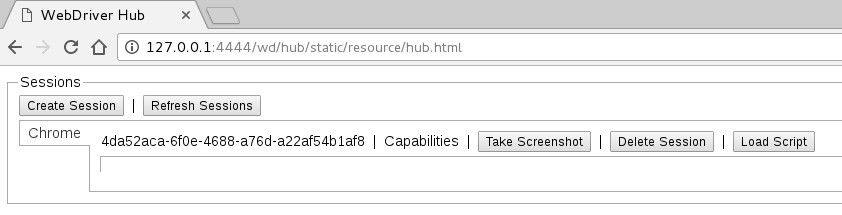
\includegraphics[scale=0.6]{registerSessionChrome}
	}
	\captionof{figure}{Registro de sesión en navegador chrome}
	\source{fuente: (Elaboración propia)}
	\label{fig:Registro de sesión en navegador chrome}
\end{minipage}

En el segmento de código \ref{lst:configSetUpChrome}, en la línea tres se
tiene que reemplazar la instrucción \textquotedouble{firefox} por \textquotedouble{chrome}.

\begin{lstlisting}[language=PHP, caption={Configuración de ejecución de prueba para chrome.}, label={lst:configSetUpChrome}]
class ContentTest extends CWebDriverTestCase {
	protected function setUp() {
        parent::setUp('localhost', 4444, 'chrome');
    }
    ...
}
\end{lstlisting}

\end{enumerate}

\end{itemize}

\section{Duración proyecto}

Definir el tiempo de un sprint en 10 días hábiles para realizar la estimación
de esfuerzo del equipo desarrollo, en consideración se utilizo 21 sprints
para definir el siguiente orden de prioridad de las historias en cuadro
\ref{tab:Product backlog - primera parte}, 
\ref{tab:Product backlog - segunda parte} y
\ref{tab:Product backlog - tercera parte}.

% first part product backlog
\begin{minipage}[!htb]{\hsize}\centering
\begin{tabular}{|l|l|l|l|l|}
\hline
\multicolumn{1}{|c|}{\textbf{Historia}} & \multicolumn{1}{c|}{\textbf{Requerimiento}} & \multicolumn{1}{c|}{\textbf{Prioridad}} & \multicolumn{1}{c|}{\textbf{Programador}} & \multicolumn{1}{c|}{\textbf{Sprint}} \\ \hline
56 & Gestión de Ocupación. & Alto & Omar & 1 \\ \hline
06 & \begin{tabular}[c]{@{}l@{}}Registro manual deusuario aprendiz a la \\ plataforma.\end{tabular} & Alto & Omar & 1 \\ \hline
20 & Implementar página maestra de plataforma. & Alto & Rudy & 0 \\ \hline
19 & \begin{tabular}[c]{@{}l@{}}Facilitar adaptación de plataforma al entorno\\ según al dispositivo.\end{tabular} & Alto & Rudy,Omar & 0 \\ \hline
05 & Registro por medio de red social. & Alto & Omar & 1 \\ \hline
10 & Identificación por medio de red social. & Alto & Omar & 1,2 \\ \hline
07 & Gestionar contenido. & Alto & Leonardo & \begin{tabular}[c]{@{}l@{}}1,2,3\\ 4,5,20\end{tabular} \\ \hline
13 & Gestionar categoría. & Alto & Omar & 2,3,20 \\ \hline
16 & \begin{tabular}[c]{@{}l@{}}Generar menú de tipos de contenido por \\ categoría.\end{tabular} & Alto & Omar & 2,3 \\ \hline
57 & Gestión tipo contenido. & Alto & Omar & 2,4 \\ \hline
25 & Gestionar contenido por interés. & Alto & Leonardo & 4 \\ \hline
18 & Gestionar tipo de preguntas. & Alto & Rudy & 4 \\ \hline
21 & Gestión rol usuario tutor. & Alto & Rudy,Omar & 3,5 \\ \hline
22 & Gestión rol usuario coordinador. & Alto & Rudy,Omar & 3,4,5 \\ \hline
14 & \begin{tabular}[c]{@{}l@{}}Gestionar mi pregunta de selección múltiple\\ de contenido.\end{tabular} & Alto & Rudy,Omar & 3,5 \\ \hline
50 & Reiniciar contraseña de usuario. & Alto & Omar & 5 \\ \hline
15 & \begin{tabular}[c]{@{}l@{}}Gestionar mi pregunta de ordenamiento \\ de contenido.\end{tabular} & Alto & Rudy & 5 \\ \hline
17 & \begin{tabular}[c]{@{}l@{}}Gestionar mi preguntas de transcripción\\ de contenido.\end{tabular} & Alto & Rudy & 5 \\ \hline
31 & \begin{tabular}[c]{@{}l@{}}Gestionar mi preguntas de comprensión\\ en contenido.\end{tabular} & Alto & Rudy,Omar & 5 \\ \hline
49 & \begin{tabular}[c]{@{}l@{}}Visualización de Pregunta tipo selección\\ múltiple front end.\end{tabular} & Alto & Rudy & 5,6 \\ \hline
32 & Gestionar mi pregunta de tipo juego en contenido. & Alto & Rudy,Omar & 6 \\ \hline
51 & \begin{tabular}[c]{@{}l@{}}Visualización de pregunta tipo rrdenamiento\\ front end.\end{tabular} & Alto & Leonardo & 5,6 \\ \hline
\end{tabular}
\captionof{table}{Product backlog - primera parte}
\source{fuente: (Elaboración propia)}
\label{tab:Product backlog - primera parte}
\end{minipage}

% second part product backlog
\begin{minipage}[!htb]{\hsize}\centering
\begin{tabular}{|l|l|l|l|l|}
\hline
\multicolumn{1}{|c|}{\textbf{Historia}} & \multicolumn{1}{c|}{\textbf{Requerimiento}} & \multicolumn{1}{c|}{\textbf{Prioridad}} & \multicolumn{1}{c|}{\textbf{Programador}} & \multicolumn{1}{c|}{\textbf{Sprint}} \\ \hline
26 & \begin{tabular}[c]{@{}l@{}}Evaluación de respuesta selección múltiple\\ en contenido.\end{tabular} & Medio & Rudy & 6,7 \\ \hline
27 & \begin{tabular}[c]{@{}l@{}}Evaluación de respuestas de ordenamiento\\ en contenido.\end{tabular} & Medio & Rudy & 7 \\ \hline
45 & \begin{tabular}[c]{@{}l@{}}Gestionar mi visualización gráfica de\\ contenido.\end{tabular} & Medio & Omar & 8,9 \\ \hline
30 & \begin{tabular}[c]{@{}l@{}}Gestionar mi pregunta de grabación en\\ contenido.\end{tabular} & Alto & Rudy,Omar & 5,9,10 \\ \hline
03 & \begin{tabular}[c]{@{}l@{}}Suscripción a un podcast de un usuario\\ aprendiz autorregulado.\end{tabular} & Medio & Omar & \begin{tabular}[c]{@{}l@{}}7,8,9,\\ 11\end{tabular} \\ \hline
11 & \begin{tabular}[c]{@{}l@{}}Animación transcripción en contenido de\\ tipo audio.\end{tabular} & Medio & Omar & 9 \\ \hline
59 & Liberación de contenidos & Medio & Omar & 9,10 \\ \hline
60 & \begin{tabular}[c]{@{}l@{}}Darse de baja suscripción podcast aprendiz\\ autorregulado.\end{tabular} & Bajo & Omar & 11 \\ \hline
44 & \begin{tabular}[c]{@{}l@{}}Animación transcripción en contenido de \\ tipo vídeo.\end{tabular} & Medio & Omar & 11 \\ \hline
64 & \begin{tabular}[c]{@{}l@{}}Relacionar transcripción con glosario en\\ contenido audio.\end{tabular} & Medio & Omar & 11 \\ \hline
32 & \begin{tabular}[c]{@{}l@{}}Visualización de pregunta tipo transcripción\\ front end.\end{tabular} & Alto & Rudy & 6,7 \\ \hline
53 & \begin{tabular}[c]{@{}l@{}}Visualización de pregunta tipo grabación\\ front end.\end{tabular} & Alto & Rudy & 8 \\ \hline
54 & \begin{tabular}[c]{@{}l@{}}Visualización de pregunta tipo comprensión\\ front end.\end{tabular} & Alto & Rudy & 8 \\ \hline
55 & \begin{tabular}[c]{@{}l@{}}Visualización de pregunta tipo juego front\\ end.\end{tabular} & Alto & Rudy & 3,8 \\ \hline
33 & \begin{tabular}[c]{@{}l@{}}Gestionar pregunta de selección múltiple\\ en contenido.\end{tabular} & Alto & Rudy, Omar & 3,5 \\ \hline
34 & \begin{tabular}[c]{@{}l@{}}Gestionar pregunta de ordenamiento en \\ contenido.\end{tabular} & Alto & Rudy, Omar & 3,5 \\ \hline
35 & \begin{tabular}[c]{@{}l@{}}Gestionar pregunta de transcripción en\\ contenido.\end{tabular} & Alto & Rudy, Omar & 3,5 \\ \hline
36 & \begin{tabular}[c]{@{}l@{}}Gestionar pregunta de grabación en\\ contenido.\end{tabular} & Alto & Rudy, Omar & \begin{tabular}[c]{@{}l@{}}3,5,\\ 9,10\end{tabular} \\ \hline
37 & \begin{tabular}[c]{@{}l@{}}Gestionar pregunta de comprensión en\\ contenido.\end{tabular} & Alto & Rudy, Omar & 3,5 \\ \hline
38 & Gestionar preguntas de juego en contenido. & Alto & Rudy & 3,6 \\ \hline
61 & Registrar glosario audio podcast. & Medio & Omar & 14 \\ \hline
64 & Registrar subtitulado podcast. & Medio & Omar & 15,16 \\ \hline
64 & Gestión traducción transcripción en podcast. & Medio & Omar & 14,15,16 \\ \hline
62 & Implementar Prueba. & Bajo & Omar & \begin{tabular}[c]{@{}l@{}}16,17,18,\\19,21\end{tabular} \\ \hline
63 & Elaborar diccionario micro-formato. & Bajo & Omar & 20 \\ \hline
39 & \begin{tabular}[c]{@{}l@{}}Reproducción de audio de comprensión en\\ contenido.\end{tabular} & Alto & Rudy, Omar & 3 \\ \hline
\end{tabular}
\captionof{table}{Product backlog - segunda parte}
\source{fuente: (Elaboración propia)}
\label{tab:Product backlog - segunda parte}
\end{minipage}

% thrid part 
\begin{minipage}[!htb]{\hsize}\centering
\begin{tabular}{|l|l|l|l|l|}
\hline
\multicolumn{1}{|c|}{\textbf{Historia}} & \multicolumn{1}{c|}{\textbf{Requerimiento}} & \multicolumn{1}{c|}{\textbf{Prioridad}} & \multicolumn{1}{c|}{\textbf{Programador}} & \multicolumn{1}{c|}{\textbf{Sprint}} \\ \hline
40 & \begin{tabular}[c]{@{}l@{}}Evaluación de pregunta de comprensión en \\ contenido.\end{tabular} & Alto & Rudy & 3 \\ \hline
12 & \begin{tabular}[c]{@{}l@{}}Representación de palabra en glosario de\\ contenido.\end{tabular} & Medio & Omar & 2 \\ \hline
41 & Visualización de sub-categoría front end. & Medio & Leonardo,Rudy & 2 \\ \hline
42 & \begin{tabular}[c]{@{}l@{}}Animación de imagen de contenido vídeo\\ lado Front End.\end{tabular} & Medio & Omar & 2,11\\ \hline
43 & Visualización de contenido front end. & Medio & Leonardo,Rudy & 2 \\ \hline
48 & Gestionar visualización gráfica de contenido. & Medio & Omar & 2,9,15 \\ \hline
28 & \begin{tabular}[c]{@{}l@{}}Evaluación de respuesta de transcripción\\ en contenido.\end{tabular} & Medio & Rudy & 2 \\ \hline
01 & Descarga de recursos dentro de contenido. & Bajo & Leonardo &  \\ \hline
02 & Comentar en contenido. & Bajo & Leonardo &  \\ \hline
29 & \begin{tabular}[c]{@{}l@{}}Visualización según ancho de banda\\ reproducción de vídeo\end{tabular} & Bajo & Leonardo &  \\ \hline
08 & \begin{tabular}[c]{@{}l@{}}Generar histograma de suscrito y visita\\ en mi contenido.\end{tabular} & Bajo & Omar &  \\ \hline
09 & \begin{tabular}[c]{@{}l@{}}Generar histograma de mis 10 contenidos\\ más visitados.\end{tabular} & Bajo & Leonardo &  \\ \hline
23 & \begin{tabular}[c]{@{}l@{}}Generar reporte suscrito y visita de\\ contenidos.\end{tabular} & Bajo & Leonardo &  \\ \hline
24 & Generar histograma de 10 contenidos. & Bajo & Leonardo &  \\ \hline
\end{tabular}
\captionof{table}{Product backlog - tercera parte}
\source{fuente: (Elaboración propia)}
\label{tab:Product backlog - tercera parte}
\end{minipage}



\chapter{Conclusiones y Recomendaciones}

Como consecuencia del proyecto de adscripción, se tiene las siguientes
conclusiones y recomendaciones.

\section{Conclusiones}

\begin{itemize}

\item Se provee de un servicio de suscripción de noticia podcast vía correo
electrónico, el cual también permite la opción al usuario de darse de baja.

\item Se sincroniza transcripción con reproductor podcast por medio de un
subtitulado.

\item Se proporciona la gestión de glosario de podcast.

\item Se agrega contenido semántico para subtitulado y representación de
glosario.

\item Se utiliza pruebas de unidad para agregar manejo de una situación no 
esperada.

\end{itemize}

\section{Recomendaciones}

\subsection{Técnicas}

\begin{itemize}

\item La configuración de inicio de sesión externo por red social requiere
de una dirección pública de IP \footnote{IP: Es el método o protocolo por el cual
se envían datos desde un ordenador a otro a través de Internet. Cada
computadora en Internet tiene al menos una dirección IP que identifica de
forma exclusiva de todos los demás ordenadores en Internet. \cite{ip}}.

\item El servidor web de producción es requerido  por parte de la unidad
patrocinadora, solicitar autorización por escrito al responsable para
la transferencia de tecnología.

\item El proyecto de adscripción de software debe utilizar licencia LPG-Bolivia,
descrito en Anexo D.

\end{itemize}

\subsection{Herramientas}

\begin{itemize}

\item El el uso de un framework \footnote{framework: Es un conjunto de
recursos y herramientas para desarrolladores de software para crear y
gestionar aplicaciones web, servicios web y sitios web. \cite{framework}}
contempla los siguientes aspectos miembros de la comunidad y curva de
aprendizaje.

\item El uso de un extractor de microformato \footnote{microformato: http://pin13.net/}
requiere disponer de un equipo con dirección pública de IP.

\item Se recomienda utilizar un canal IRC 
\footnote{IRC: irc://irc.freenode.net/microformats} como medio de comunicación
para solicitar sugerencia y uso de microformato.

\item El uso de herramientas colaborativas de control de versión de código
(git) y manejadores de tarea (pivotal tracker) ofrece soporte de trabajo
entre personas.

\item Utilizar un servidor web de producción como ambiente de pruebas para tareas
de segundo plano y servicio de correo.

\end{itemize}

\subsection{Postular a proyecto de adscripción}

\begin{itemize}

\item los términos de referencia deben ser elaborados por la unidad
patrocinadora, caso contrario el equipo de informática tiene que realizar
entrevistas con el responsable del proyecto

\end{itemize}

\subsection{Proceso proyecto de adscripción}

\begin{itemize}

\item Las autoridades de un proyecto deben realizar una reunión de
presentación, Además de dar a conocer el estado de avance.

\item El equipo de desarrollo debe disponer de una ejemplar original de
documentos de términos de referencia, historias de usuario, documento de
validación y aceptación.

\item El tutor y el equipo de desarrollo deben disponer de un ambiente de
trabajo.

\end{itemize}

\subsection{Conclusión proyecto de adscripción}

\begin{itemize}

\item Equipo desarrollo debe solicitar una carta de conclusión de proyecto
dirigida la autoridad responsable de la unidad patrocinadora adjuntando
copia de los documentos de validación y aceptación.

\end{itemize}

\subsection{Redacción}

\begin{itemize} 

\item Un documento de redacción de adscripción debe contemplar reglas
gramaticales de ortografía, coherencia y concordancia por lo cual se debe
solicitar colaboración a una persona del área de LAEL.

\item Concluida la redacción del Capítulo 5 (Conclusiones y Recomendaciones),
se recomienda estructurar el Capítulo 1 (Introducción).

\item Las figuras de elaboración propia deben ser escritas en lenguaje 
español.

\end{itemize}

\subsection{Proceso de trabajo en equipo desarrollo}

\begin{itemize}

\item El equipo de desarrollo debe utilizar las habilidades de disciplina,
responsabilidad y honestidad.

\item El equipo de desarrollo debe utilizar estándares de trabajo de convención
de variable, nombre de la función, lenguaje a utilizar y herramientas de
soporte de manera que se elabore un documento como reglamento interno.

\end{itemize}

\section{Trabajos futuros}

Se recomienda las siguientes experiencias para proyectos similares.

\begin{itemize}

\item Un proyecto de adscripción es considerado como un proyecto de grado
por contemplar de un cliente real, aplicación de conocimiento en ciencias de
la computación y propuesta de solución a un problema específico.

\item Si se trata de un proyecto digital se sugiere utilizar servidores web 
especializados como nginx \footnote{ngnix: Es conocido por su alto 
rendimiento, la estabilidad, la gran variedad de funciones, configuración
simple, y bajo consumo de recursos. \cite{nginx}}  o lighttpd \footnote{lighttpd: 
Esta diseñado y optimizado para entornos de alto rendimiento. Con una 
pequeña huella de memoria en comparación con otros servidores web, la
gestión eficaz de la CPU de carga y avanzando lighttpd conjunto de 
características es la solución perfecta para cada servidor que está
sufriendo problemas de carga. \cite{lighttps}}.
 
\item Crear material digital como de imagen, historieta y producción de
audio/vídeo utilizar software open source \footnote{open source: Es software
cuyo código fuente está disponible para su modificación o mejora por parte
de nadie. \cite{openSource}}, el software open source brinda las siguientes
características de multiplataforma y optimiza recursos para realizar
transmisión para ancho de banda limitado.

\end{itemize}

\bibliography{bib/Literature}

% remove empty page after appendix
\cleardoublepage\makeatletter\@openrightfalse\makeatother

\appendix
\addappheadtotoc
\appendixpage

\chapter{Diagrama Entidad Relación}

\begin{minipage}{1.0\textwidth}
	\centering
	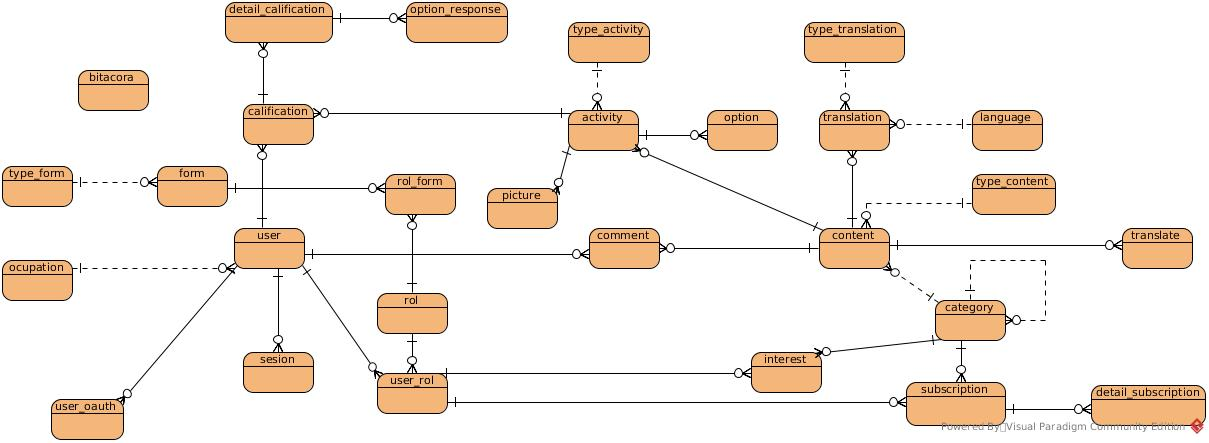
\includegraphics[angle=90, scale=0.4]{modelDatabase}
	\captionof{figure}{Modelo Base de Datos}
	\source{fuente: (Elaboración Propia)}
\end{minipage}


\chapter{Documento de validación y aceptación 04-11-2014}

El presente documento tiene por finalidad el de constatar la conformidad tanto
del Cliente como el equipo de desarrollo.

Esta es la presentación de la versión alpha estipulado en la propuesta
técnica presentada Correspondiente al Sprint primero \textquotedblleft 
Versión Alpha listo\textquotedblright.

Dicha presentación está sujeto al pago del 17 (por ciento) del total del
costo del sistema, para Mayor conformidad para ambas partes se remarca los
siguientes aspectos.

\begin{enumerate}

\item \textbf{Escala de evaluación}

\begin{table}[!h]
\centering
\begin{tabular}{|c|c|c|}
\hline
\textbf{Punta je} & \textbf{Valor Numérico} & \textbf{Concepto} \\ \hline
NA & 0 & \begin{tabular}[c]{@{}c@{}}Se necesita hacer cambios\\ profundos\end{tabular} \\ \hline
RA & 1 & \begin{tabular}[c]{@{}c@{}}Requiere modificación para\\ aceptar\end{tabular} \\ \hline
A & 2 & Aceptado \\ \hline
\end{tabular}
\end{table}

\item \textbf{Las funcionalidades a presentar son las siguientes:}

\begin{itemize}

	\item Registro manual de usuario aprendiz a la plataforma.
		\begin{itemize}
			\item Envió de solicitud de confirmación de correo electrónico a bandeja de entrada.
			\item Modificar datos personales.
		\end{itemize}
	\item Registro por medio de red social.
		\begin{itemize}
			\item Registro por Facebook.
			\item Registro por Google.
			\item Registro por Twitter.
		\end{itemize}
	\item Implementar Página Maestra de Plataforma.

\end{itemize}

\item El pago del 17 (por ciento) se dará por hecho si se está conforme 
con 3 de las 4 funcionalidades.

\end{enumerate}

Se está conforme con una funcionalidad si se cumple los siguientes aspectos
estipulados en el sumario de evaluación de párrafos.

\section{Sumario de Evaluación de Parámetro}

\subsection{Registro manual de usuario aprendiz a la plataforma}

\textbf{Envió de solicitud de confirmación de correo electrónico a
bandeja de entrada}

Envió de solicitud de confirmación de correo electrónico a bandeja
de entrada. Abra un navegador web con la siguiente dirección (URL): plataforma
\footnote{plataforma: http:// plataformaeducativalael.hum.umss.edu.bo}, pinche en 
el enlace Registrar ubicado en la parte superior derecha.

\begin{table}[!htb]
\centering
\begin{tabular}{|l|l|l|}
\hline
\multicolumn{1}{|c|}{\textbf{N}} & \multicolumn{1}{c|}{\textbf{Parametros a evaluar}} & \multicolumn{1}{c|}{\textbf{Puntaje}} \\ \hline
01 & \begin{tabular}[c]{@{}l@{}}\textquestiondown Ud. puede ingresar datos en los campos y realizar clic en el botón\\ Registrar: Dirección de Correo, Nombre de Usuario, Contraseña, Repetir\\ Contraseña, Seleccione un valor de Ocupación, Sub Ocupación, Captcha?\end{tabular} &  \\ \hline
02 & \begin{tabular}[c]{@{}l@{}}\textquestiondown Ud. puede leer un mensaje \textquotedouble{Un correo electrónico que contiene m\'{a}s\\ instrucciones ha sido enviada bandeja de dirección de correo electrónico\\ proveedor}?\end{tabular} &  \\ \hline
03 & \begin{tabular}[c]{@{}l@{}}\textquestiondown Ud. ingrese a su cuenta de correo con la cual se registró anteriormente,\\ revise en bandeja spam, un mensaje de Administrador en el cuerpo un\\ enlace de confirmación?\end{tabular} &  \\ \hline
04 & \begin{tabular}[c]{@{}l@{}}\textquestiondown Ud. puede pinchar en el enlace y mostrarle el siguiente mensaje \textquotedouble{Su\\ dirección de correo electrónico ha sido verificado exitosa mente}, en la\\ parte superior de inicio sesión?\end{tabular} &  \\ \hline
\end{tabular}
\end{table}

Nota: Si está conforme con la funcionalidad \textquotedouble{Envió de
solicitud de confirmación de correo electrónico a bandeja de entrada}
si la sumatoria de Puntaje tiene un valor mayor y/o igual 5.

Las siguientes funcionalidades se realizan con credenciales propias.

\textbf{Modificar datos personales}

En la presentación principal en la parte superior derecha se tiene un enlace 
Inicio Sesión, pinchar sobre el mismo y mostrara una ventana de autentificar
con los siguientes campos: Nombre de Usuario, Contraseña.

\begin{table}[!htb]
\centering
\begin{tabular}{|l|l|l|}
\hline
\multicolumn{1}{|c|}{\textbf{N}} & \multicolumn{1}{c|}{\textbf{Parámetros a evaluar}} & \multicolumn{1}{c|}{\textbf{Puntaje}} \\ \hline
01 & \begin{tabular}[c]{@{}l@{}}\textquestiondown Ud. pude visualizar un Panel Administrativo en donde si tiene un mensaje\\ \textquotedouble{Hola} acompañado de su nombre de usuario en la parte superior derecha?\end{tabular} &  \\ \hline
02 & \begin{tabular}[c]{@{}l@{}}\textquestiondown Ud. puede visualizar un sus datos personales pinchando sobre la imagen\\ de una persona ubicada en la esquina superior derecha y presionar la\\ opción Perfil?\end{tabular} &  \\ \hline
03 & \begin{tabular}[c]{@{}l@{}}\textquestiondown Ud. puede editar sus datos personales pinchando en el enlace \textquotedouble{Actualizar\\ Usuario} ubicado en la parte inferior\end{tabular} &  \\ \hline
04 & \begin{tabular}[c]{@{}l@{}}\textquestiondown Ud. puede salvar sus datos pinchando en el bot\'{o}n \textquotedouble{Salvar} sobre el\\ c\'{o}digo verificación?\end{tabular} &  \\ \hline
05 & \begin{tabular}[c]{@{}l@{}}\textquestiondown Ud. puede cerrar sesión haciendo clic en la imagen del hombre cito\\ ubicado en la parte superior derecha del Panel Administrativo la opción\\ Cerrar Sesión?\end{tabular} &  \\ \hline
\end{tabular}
\end{table}

Nota: Si está conforme con la funcionalidad \textquotedouble{Modificar 
datos personales} si la sumatoria de Puntaje tiene un 
valor igual o mayor 6.

\section{Registro por medio de red social}

En la presentación principal en la parte superior derecha se tiene un enlace 
Inicio Sesión, pinchar sobre el mismo y mostrara una ventana de autentificar
con los siguientes enlaces:

\begin{itemize}
	\item Ingresar con Google.
	\item Ingresar con Facebook.
	\item Ingresar con Twitter.
\end{itemize}

Tomar en cuenta que para esta funcionalidad de registro por medio de red social
es con una cuenta de correo utilizada por primera vez en el sistema.

\begin{table}[!htb]
\centering
\begin{tabular}{|l|l|l|}
\hline
\multicolumn{1}{|c|}{\textbf{N}} & \multicolumn{1}{c|}{\textbf{Parametros a evaluar}} & \multicolumn{1}{c|}{\textbf{Puntaje}} \\ \hline
01 & \begin{tabular}[c]{@{}l@{}}\textquestiondown Ud. puede Registrarse pinchando sobre el bot\'{o}n Ingresar con Google\\ llenar con sus credenciales y un evento Login, le muestra un Panel\\ Administrativo donde en la parte superior derecha superior se muestra\\ su correo electrónico?\end{tabular} &  \\ \hline
02 & \begin{tabular}[c]{@{}l@{}}\textquestiondown Ud. puede cerrar sesión haciendo clic en la imagen del hombre cito\\ ubicado en la parte superior derecha del Panel Administrativo la opción\\ Cerrar Sesión?\end{tabular} &  \\ \hline
03 & \begin{tabular}[c]{@{}l@{}}\textquestiondown Ud. puede Registrarse pinchando sobre el bot\'{o}n Ingresar con Facebook\\ y llenando las credenciales de la red social y pinchando en el bot\'{o}n Login,\\ entonces le muestra un Panel Administrativo donde en la parte superior\\ derecha superior se muestra su correo electrónico?\end{tabular} &  \\ \hline
04 & \begin{tabular}[c]{@{}l@{}}\textquestiondown Ud. puede cerrar sesión haciendo clic en la imagen del hombre cito\\ ubicado en la parte superior derecha del Panel Administrativo la opción\\ Cerrar Sesión?\end{tabular} &  \\ \hline
05 & \begin{tabular}[c]{@{}l@{}}\textquestiondown Ud. puede Registrarse pinchando sobre el bot\'{o}n Ingresar con Twitter\\ llenar con sus credenciales y un evento Sign in luego dándole permiso de\\ autorización, le muestra un Panel Administrativo donde en la parte superior\\ derecha superior se muestra su correo electrónico?\end{tabular} &  \\ \hline
06 & \begin{tabular}[c]{@{}l@{}}\textquestiondown Ud. puede cerrar sesión haciendo clic en la imagen del hombre cito\\ ubicado en la parte superior derecha del Panel Administrativo la opción\\ Cerrar Sesión?\end{tabular} &  \\ \hline
\end{tabular}
\end{table}

Nota: Si está conforme con la funcionalidad \textquotedouble{Registro por 
medio de red social} si la sumatoria de Puntaje tiene un
valor mayor igual 6.

\section{Implementar página maestra de plataforma}

\begin{minipage}[!htb]{\hsize}\centering
\begin{tabular}{|l|l|l|}
\hline
\multicolumn{1}{|c|}{\textbf{N}} & \multicolumn{1}{c|}{\textbf{Parametros a evaluar}} & \multicolumn{1}{c|}{\textbf{Puntaje}} \\ \hline
01 & \begin{tabular}[c]{@{}l@{}}\textquestiondown Ud. puede reproducir un vídeo pinchando sobre la imagen \textquotedouble{VER\\ PRESENTACIÓN} ubicada en la parte superior de la Página Maestra?\end{tabular} &  \\ \hline
02 & \begin{tabular}[c]{@{}l@{}}\textquestiondown Ud. puede Registrarse pinchando sobre el bot\'{o}n Ingresar con Google\\ llenar con sus credenciales y un evento Login, le muestra un Panel\\ Administrativo donde en la parte inferior de Inicio, se muestra su correo\\ electrónico?\end{tabular} &  \\ \hline
\end{tabular}
\end{minipage}

Nota: Si está conforme con la funcionalidad \textquotedouble{Implementar 
Página Maestra de Plataforma} si la sumatoria de Puntaje tiene un valor 2.

Si se cumple el punto 3 procedemos a firmar este documento los representantes
para su aceptación.

\begin{minipage}[!htb]{\hsize}\centering
\begin{tabular}{|l|l|}
\hline
\begin{tabular}[c]{@{}l@{}}..........................................\\ Lic. Manuel Camacho Arce\\ PRODUCT OWNER\end{tabular} & \begin{tabular}[c]{@{}l@{}}.........................................\\ Juan Omar Huanca Balboa\\ SCRUM MASTER\end{tabular} \\ \hline
\end{tabular}
\end{minipage}

\chapter{Documento de validación y aceptación 26-01-2015}

El presente documento tiene por finalidad de constatar la conformidad tanto del
Cliente como el equipo de desarrollo.

Esta es la presentación de la versión Alpha estipulado en la propuesta 
técnica presentada Correspondiente al Sprint segundo, tercero \textquotedouble{
Versión Alpha listo}.

Dicha presentación está sujeto al pago del 4 (por ciento) del total del
costo del sistema, para Mayor conformidad para ambas partes se remarca los 
siguientes aspectos.

\begin{enumerate}

\item \textbf{Escala de evaluación}

\begin{table}[!h]
\centering
\begin{tabular}{|c|c|c|}
\hline
\textbf{Puntaje} & \textbf{Valor Numérico} & \textbf{Concepto} \\ \hline
NA & 0 & \begin{tabular}[c]{@{}c@{}}Se necesita hacer cambios\\ profundos\end{tabular} \\ \hline
RA & 1 & \begin{tabular}[c]{@{}c@{}}Requiere modificación para\\ aceptar\end{tabular} \\ \hline
A & 2 & Aceptado \\ \hline
\end{tabular}
\end{table}

\item \textbf{Las funcionalidades a presentar son las siguientes:}

\begin{itemize}

	\item Reiniciar Contraseña de Usuario (Usuario habilitado).
		\begin{itemize}
			\item Envió de solicitud de cambio de contraseña.
		\end{itemize}
	\item Gestión rol usuario Coordinador (Usuario habilitado).
	\item Gestionar Categoría (Usuario autentificado).
	\item Gestión rol usuario Tutor(Usuario habilitado, Sub categoría creada).
	\item Gestionar Contenido por intereses(Tener rol Tutor, Estar asignado a 
	sub categoría).
	\item Generar menú de tipos de contenido por Categoría(Contenido publicado).
		
\end{itemize}

\item \textbf{El pago del 4 (por ciento) se dar\'{a} por hecho si se está conforme 
con la mitad más uno de los puntos}

\end{enumerate}

Si está conforme con una funcionalidad si se cumple los siguientes aspectos
estipulados en el sumario de evaluación de párrafos.

\section{Sumario de Evaluación de parámetro}

\subsection{Reiniciar Contraseña de Usuario}

\textbf{Envió de solicitud de cambio de contraseña}

Requisito: Ser usuario habilitado, caso contrario utilizar las credenciales del
usuario por defecto; usuario: Juan Omar Huanca Balboa contraseña: autorregulado.

Abra un navegador web con la siguiente dirección (URL): plataforma 
\footnote{plataforma: http:// plataformaeducativalael.hum.umss.edu.bo} Pinche en
el enlace Iniciar Sesión ubicado en la parte superior derecha, seguido de
pinchar sobre en enlace Recuperar Contraseña.

\begin{minipage}[b]{\hsize}\centering
\begin{tabular}{|l|l|l|}
\hline
\multicolumn{1}{|c|}{\textbf{N}} & \multicolumn{1}{c|}{\textbf{Parametros a evaluar}} & \multicolumn{1}{c|}{\textbf{Puntaje}} \\ \hline
01 & \begin{tabular}[c]{@{}l@{}}Si Ud. eligió la cuenta por defecto llene, correo:\\ omar.huanca.balboa@gmail.com, contraseña:\\ omar.huanca.balboa. Captcha, pinchar sobre el bot\'{o}n Enviar\\ entonces ejecutar paso 03; caso contrario ingrese el correo\\ electrónico relacionado con la cuenta habilitada.\end{tabular} &  \\ \hline
02 & \begin{tabular}[c]{@{}l@{}}\textquestiondown Ud. puede ingresar datos en los campos: Dirección de Correo,\\ Captcha pinchar sobre el botón Enviar ?\end{tabular} &  \\ \hline
03 & \begin{tabular}[c]{@{}l@{}}\textquestiondown Ud. puede leer un mensaje \textquotedblleft Un correo electrónico que\\ contiene m\'{a}s instrucciones ha sido enviada bandeja de dirección\\ de correo electrónico asociada con su cuenta de proveedor\textquotedblright ?\end{tabular} &  \\ \hline
04 & \begin{tabular}[c]{@{}l@{}}\textquestiondown Ud. ingrese a su bandeja de mensajes del correo electrónico\\ ingresado anteriormente, un mensaje de Administrador -\\ Recuperar Contraseña en el cuerpo un enlace?\end{tabular} &  \\ \hline
05 & \begin{tabular}[c]{@{}l@{}}\textquestiondown Ud. pinche sobre el enlace le enviara a un formulario con los\\ siguientes campos: Contraseña, Repetir Contraseña?\end{tabular} &  \\ \hline
06 & \begin{tabular}[c]{@{}l@{}}\textquestiondown Ud. ingrese la nueva contraseña dos veces en los campos:\\ Contraseña, Repetir Contraseña y pinchar sobre el bot\'{o}n Enviar,\\ le muestra el siguiente mensaje \textquotedblleft Su dirección de correo ha sido\\ verificado\textquotedblright ?\end{tabular} &  \\ \hline
07 & \begin{tabular}[c]{@{}l@{}}\textquestiondown Si Ud. eligió la cuenta de usuario por defecto (autorregulado)\\ entonces ingrese la nueva contraseña pinche sobre el bot\'{o}n\\ Iniciar Sesión con sus nuevas credenciales caso contrario\\ ingrese la cuenta de usuario de la cuenta habilitada?\end{tabular} &  \\ \hline
\end{tabular}
\end{minipage}

Nota: Si está conforme con la funcionalidad \textquotedouble{Recobrar Contraseña} si la sumatoria
de Puntaje tiene un valor mayor y/o igual 4.

Las siguiente funcionalidad tiene que solicitar webmaster (administrador) que
agregue el rol coordinador en una cuenta habilitada, caso contrario puede hacer
uso de la cuenta por defecto nombre usuario: coordinador, contraseña: 
coordinador.

Ingrese la siguiente dirección URL en su navegador: plataforma 
\footnote{plataforma: http:// plataformaeducativalael.hum.umss.edu.bo}

Pinche en el enlace Iniciar Sesión ubicado en la parte superior derecha

\section{Gestión rol usuario Coordinador}

\begin{minipage}[b]{\hsize}\centering
\begin{tabular}{|l|l|l|}
\hline
\multicolumn{1}{|c|}{\textbf{N}} & \multicolumn{1}{c|}{\textbf{Parámetros a evaluar}} & \multicolumn{1}{c|}{\textbf{Puntaje}} \\ \hline
01 & \begin{tabular}[c]{@{}l@{}}\textquestiondown Si Ud. Eligió la cuenta habilitada tiene que dar a conocer al\\ webmaster a cual sub categor\'{i}a quiere estar asignado (Quechua \\ Básico, Quechua Psicosocial, Francés Básico, English Spread in \\ Cochabamba)? \\ \end{tabular} &  \\ \hline
02 & \begin{tabular}[c]{@{}l@{}}\textquestiondown Ud. Inicie sesión con las credenciales de la cuenta habilitada,\\ 
deber\'{i}a de aparecer nuevas opciones en el menú derecho de su \\ página principal de sesión?\end{tabular} &  \\ \hline
03 & \begin{tabular}[c]{@{}l@{}}\textquestiondown Ud. Puede solicitar al webmaster verbalmente que se pueden\\ revocar los privilegios asignados a la cuenta habilitada\\ mencionada anteriormente?\end{tabular} &  \\ \hline
\end{tabular}
\end{minipage}

Nota: Si está conforme con la funcionalidad \textquotedouble{Gestión 
rol usuario Coordinador} si la sumatoria de Puntaje tiene un
valor mayor y/o igual 2.

La siguiente funcionalidad tiene ingresar con una cuenta habilitada que tenga 
el rol de coordinador asignado correspondientemente. Caso contrario ingrese con
las credenciales Nombre Usuario: coordinador, Contraseña: coordinador.

Ingrese la siguiente dirección URL en su navegador: plataforma 
\footnote{plataforma: http:// plataformaeducativalael.hum.umss.edu.bo}
o pinche sobre la opción Inicio ubicado en el menú principal de la 
página de presentación Principal.

Pinche en el enlace Iniciar Sesión ubicado en la parte superior derecha.

\section{Gestionar Categoría}

\begin{minipage}[b]{\hsize}\centering
\begin{tabular}{|l|l|l|}
\hline
\multicolumn{1}{|c|}{\textbf{N}} & \multicolumn{1}{c|}{\textbf{Parámetros a evaluar}} & \multicolumn{1}{c|}{\textbf{Puntaje}} \\ \hline
01 & \begin{tabular}[c]{@{}l@{}}\textquestiondown Ud. Ingrese sus credenciales en los campos: Nombre Usuario,\\ Contraseña, le aparecer\'{a} una opción de su cuenta\\ administrativa?\end{tabular} &  \\ \hline
02 & \begin{tabular}[c]{@{}l@{}}\textquestiondown Ud. Pinche sobre la opción Categoría en la sub opción\\ Registrar Categoría y le muestra un formulario?\end{tabular} &  \\ \hline
03 & \begin{tabular}[c]{@{}l@{}}\textquestiondown Ud. Ingrese el nombre de la categoría padre con la categoría\\ 
reflexiva opción Padre, Archivo Respuesta Correcta, Archivo\\ Respuesta Incorrecta, pinchar sobre el bot\'{o}n Registrar, a\\
continuación deber\'{i}a mostrarle un detalle de la categoría padre\\ registrada?\end{tabular} &  \\ \hline
04 & \begin{tabular}[c]{@{}l@{}}\textquestiondown Ud. Pinche sobre la opción Categoría en la sub opción\\ Registrar Categoría y le muestra un formulario?\end{tabular} &  \\ \hline
05 & \begin{tabular}[c]{@{}l@{}}\textquestiondown Ud. Ingrese el nombre de la categoría hija con la categoría\\ reflexiva opción Hijo, Nivel Categoría, Imagen Categoría,\\ Descripción Categoría, Descripción Créditos, Descripción\\ Objetivos, pinchar sobre el botón Registrar, a continuación\\ debería mostrarle un detalle de la categoría hijo registrado?\end{tabular} &  \\ \hline
06 & \begin{tabular}[c]{@{}l@{}}\textquestiondown Ud. Pinche sobre la opción Categoría en la sub opción\\ Administrar Categoría y le muestra una tabla de categorias\\ registradas?\end{tabular} &  \\ \hline
07 & \begin{tabular}[c]{@{}l@{}}\textquestiondown Ud. elija una opción de la tabla, seguido podrá aplicar las\\ siguiente funcionalidades: Ver, Actualizar, Eliminar. Como\\ primera opción pinche sobre la opción Ver ubicado en la parte\\ derecha bajo la etiqueta Acción, podrá observar un detalle de los\\ campos con que cuenta la categoría?\end{tabular} &  \\ \hline
08 & \begin{tabular}[c]{@{}l@{}}\textquestiondown Ud. Pinche sobre la opción Categoría en la sub opción\\ Administrar Categoría y le muestra una tabla de categorías\\ registradas? \end{tabular} & \\ \hline
09 & \begin{tabular}[c]{@{}l@{}}\textquestiondown Ud. elija una opción de la tabla, como segunda opción pinche\\ sobre la acción Actualizar ubicado en la parte derecha bajo la\\ etiqueta Acción, podrá editar los campos previamente\\ registrados?\end{tabular} & \\ \hline
10 & \begin{tabular}[c]{@{}l@{}}\textquestiondown Ud. Pinche sobre la opción Categoría en la sub opción\\ Administrar Categoría y le muestra una tabla de categorías\\ registradas?\end{tabular} & \\ \hline
11 & \begin{tabular}[c]{@{}l@{}}\textquestiondown Ud elija una opción de la tabla, como tercera opción pinche\\ sobre la opción acción Borrar ubicado en la parte derecha bajo\\ la etiqueta Acción, un mensaje de confirmación le saldrá\\ pidiéndole aceptar o denegar?\end{tabular} & \\ \hline
12 & \begin{tabular}[c]{@{}l@{}}\textquestiondown Ud. Pinche sobre la opción Categoría en la sub opción\\ Administrar Categoría y le muestra una tabla de categorías\\ registradas?\end{tabular} & \\ \hline
13 & \begin{tabular}[c]{@{}l@{}}\textquestiondown Ud. Pinche sobre la opción Categoría en la sub opción Listar\\ Categoría y le muestra una lista de categorías registradas?\end{tabular} & \\ \hline
14 & \begin{tabular}[c]{@{}l@{}}\textquestiondown Ud. Podrá ordenar las categorías según el siguiente criterio:\\ Nombre Categoría, ubicado en la parte superior, inferior de la\\ lista?\end{tabular} & \\ \hline
\end{tabular}
\end{minipage}

Nota: Si está conforme con la funcionalidad \textquotedouble{Gestionar 
Categoría} si la sumatoria de Puntaje tiene un valor 
mayor y/o igual 7.

Las siguiente funcionalidad tiene que solicitar webmaster (administrador) que 
agregue el rol tutor en una cuenta habilitada, caso contrario puede hacer uso
de la cuenta por defecto nombre usuario: tutor, contraseña: tutor.

Ingrese la siguiente dirección URL en su navegador: plataforma 
\footnote{plataforma: http:// plataformaeducativalael.hum.umss.edu.bo} o pinche 
sobre la opción Inicio ubicado en el menú principal de la página 
de presentación Principal.

Pinche en el enlace Iniciar Sesión ubicado en la parte superior derecha.

\section{Gestión rol usuario Tutor}

\begin{minipage}[b]{\hsize}\centering
\begin{tabular}{|l|l|l|}
\hline
\multicolumn{1}{|c|}{\textbf{N}} & \multicolumn{1}{c|}{\textbf{Parámetros a evaluar}} & \multicolumn{1}{c|}{\textbf{Puntaje}} \\ \hline
01 & \begin{tabular}[c]{@{}l@{}}\textquestiondown Si Ud. Eligió la cuenta habilitada tiene que dar a conocer al\\ webmaster a cual sub categoría quiere estar asignado para poder\\  gestionar sus contenidos?\end{tabular} &  \\ \hline
02 & \begin{tabular}[c]{@{}l@{}}\textquestiondown Ud. Inicie sesión con las credenciales de la cuenta habilitada,\\ 
deber\'{i}a de aparecer las opciones en el menú derecho de su\\ página principal de sesión con los nombres: Mis Contenidos,\\ Actividad?\end{tabular} &  \\ \hline
03 & \begin{tabular}[c]{@{}l@{}}\textquestiondown Ud. Puede solicitar al webmaster verbalmente que se pueden\\ revocar los privilegios asignados a la cuenta habilitada\\ mencionada anteriormente?\end{tabular} &  \\ \hline
\end{tabular}
\end{minipage}

Nota: Si está conforme con la funcionalidad \textquotedouble{Gestión
rol usuario Tutor} si la sumatoria de Puntaje tiene un valor
mayor y/o igual 2.

Para realizar la siguiente funcionalidad, tiene que cumplir con la anterior
funcionalidad (Gestión rol usuario Tutor).

Ingrese la siguiente dirección URL en su navegador: plataforma 
\footnote{plataforma: http:// plataformaeducativalael.hum.umss.edu.bo} o pinche
sobre la opción Inicio ubicado en el menú principal de la página de 
presentación Principal.

Pinche en el enlace Iniciar Sesión ubicado en la parte superior derecha.

\section{Gestionar Contenido por intereses}

\begin{minipage}[b]{\hsize}\centering
\begin{tabular}{|l|l|l|}
\hline
\multicolumn{1}{|c|}{\textbf{N}} & \multicolumn{1}{c|}{\textbf{Parámetros a evaluar}} & \multicolumn{1}{c|}{\textbf{Puntaje}} \\ \hline
01 & \begin{tabular}[c]{@{}l@{}}\textquestiondown Ud. Ingrese sus credenciales en los campos: Nombre Usuario,\\ Contraseña, le aparecer\'{a} una opción de su cuenta\\ administrativa?\end{tabular} &  \\ \hline
02 & \begin{tabular}[c]{@{}l@{}}\textquestiondown Ud. Pinche sobre la opción Mis Contenidos a en la sub opción\\ Registrar Mi Contenido y le muestra un formulario?\end{tabular} &  \\ \hline
03 & \begin{tabular}[c]{@{}l@{}}\textquestiondown Ud. Ingrese el Título, Archivo Imagen, Seleccione el tipo de\\ contenido, Archivo Reproductor, Seleccione la sub categoría,\\ Fecha de liberación, Resumen, Archivo Resolución(*), Archivo\\ Glosario, Archivo Diccionario, Créditos pinchar sobre el botón\\ Registrar,a continuación debería mostrarle un detalle de la\\ categoría padre registrada?\end{tabular} &  \\ \hline
04 & \begin{tabular}[c]{@{}l@{}}\textquestiondown Ud. Pinche sobre la opci\'{o}n Mis Contenidos en la sub opción\\ Administrar Mis Contenidos y le muestra una tabla de\\ contenidos registradas?\end{tabular} &  \\ \hline
05 & \begin{tabular}[c]{@{}l@{}}\textquestiondown Ud. elija una opci\'{o}n de la tabla, como segunda opción pinche\\ sobre la acción Actualizar ubicado en la parte derecha bajo la\\ etiqueta Acción, podrá editar los campos previamente\\ registrados?\end{tabular} &  \\ \hline
06 & \begin{tabular}[c]{@{}l@{}}\textquestiondown Ud. Pinche sobre la opción Mis Contenidos en la sub opción\\ Administrar Mis Contenidos y le muestra una tabla de\\ contenidos registradas?\end{tabular} &  \\ \hline
07 & \begin{tabular}[c]{@{}l@{}}\textquestiondown Ud elija una opción de la tabla, como tercera opción pinche\\ sobre la opción acción Borrar ubicado en la parte derecha bajo\\ la etiqueta Acción, un mensaje de confirmación le saldrá\\ pidiéndole aceptar o denegar?\\\end{tabular} &  \\ \hline
08 & \begin{tabular}[c]{@{}l@{}}\textquestiondown Ud. Pinche sobre la opción Mis Contenidos en la sub opción\\ Listar Mis Contenidos y le muestra una lista de todos los\\ contenidos registrados? \end{tabular} & \\ \hline
09 & \begin{tabular}[c]{@{}l@{}}\textquestiondown Ud. Podra ordenar las categorías según el siguiente criterio:\\ Título, Fecha creación, Fecha liberación?\end{tabular} & \\ \hline
\end{tabular}
\end{minipage}

(*) Si usted define como tipo de contenido audio este campo es requerido.

Nota: Si está conforme con la funcionalidad \textquotedouble{Gestionar 
Contenido por intereses} si la sumatoria de Puntaje tiene un 
valor mayor y/o igual 5.

Ingrese la siguiente dirección URL en su navegador: plataforma 
\footnote{plataforma: http:// plataformaeducativalael.hum.umss.edu.bo} o pinche
sobre la opción Inicio ubicado en el men\'{u} principal de la página de 
presentación Principal o pinche sobre la opción Vista Página Principal
situado en la parte superior de su panel administrativo de su cuenta.

\section{Generar menú de tipos de contenido por Categoría}

\begin{minipage}[b]{\hsize}\centering
\begin{tabular}{|l|l|l|}
\hline
\multicolumn{1}{|c|}{\textbf{N}} & \multicolumn{1}{c|}{\textbf{Parámetros a evaluar}} & \multicolumn{1}{c|}{\textbf{Puntaje}} \\ \hline
01 & \begin{tabular}[c]{@{}l@{}}\textquestiondown Ud. Pinche sobre el tipo de categoría Audio/Vídeo si fuera el\\ caso con anterioridad, saldrá un elemento respecto la categoría\\  padre, pinche sobre el mismo y podrá ver una lista de sub\\ categorías asignadas al correspondiente idioma?\end{tabular} &  \\ \hline
02 & \begin{tabular}[c]{@{}l@{}}\textquestiondown Ud. Pinche sobre la imagen u/o nombre de la sub categoría ,\\
para poder ver contenido(s) creados relacionados con sub\\ categoría?\end{tabular} &  \\ \hline
03 & \begin{tabular}[c]{@{}l@{}}\textquestiondown Ud. Podrá ver una animación de desplazamiento de izquierda a\\ derecha de los contenidos comprendidos en la sub categoría, en\\ la parte inferior podrá ver los créditos y objetivos de todos los\\ episodios?\end{tabular} &  \\ \hline
\end{tabular}
\end{minipage}

Nota: Si está conforme con la funcionalidad \textquotedouble{Generar 
menú de tipos de contenido por Categoría} si la 
sumatoria de Puntaje tiene un valor mayor y/o igual 2.

Si se cumple más de los 4 puntos de 6 que fueron presentados a 
continuación procedemos a firmar este documento los representantes para su
aceptación.

\begin{minipage}[b]{\hsize}\centering
\begin{tabular}{|l|l|}
\hline
\begin{tabular}[c]{@{}l@{}}..........................................\\ Lic. Manuel Camacho Arce\\ PRODUCT OWNER\end{tabular} & \begin{tabular}[c]{@{}l@{}}.........................................\\ Juan Omar Huanca Balboa\\ SCRUM MASTER\end{tabular} \\ \hline
\end{tabular}
\end{minipage}


\cleardoublepage\makeatletter\@openrighttrue\makeatother

\chapter{Licencia Pública General v.1} \label{chap:LPG-Bolivia}

\section{Introducción}

Según \cite{LPGBolivia} esta licencia está basada en la Licencia Pública
General GNU (GNU GPL) de la Fundación para el Software Libre (www.fsf.org),
la cual ha sida adaptada por la agencia para el Desarrollo de la Sociedad de
la Información en Bolivia (ADSIB) a la normativa legal vigente en Bolivia,
enmarcada en la Ley General de Telecomunicaciones, Tecnologías de la
Información y Comunicación, Ley 164 de 8 de agosto de 2011 y el Reglamento
por el Decreto Supremo 1793 de 13 de Noviembre de 2013.
 
\section{Preámbulo}

Según \cite{LPGBolivia} hablar de software libre, se refiere a la libertar
de acción, no de precio. La LPG-Bolivia esta diseñada para garantizar la.
libertad de distribuir copias de software libre (cobrar por ello si quiere).
Los desarrollado-res que usan la LPG-Bolivia protegen tus derechos con dos
pasos: 

\begin{itemize}

\item haciendo valer el derecho de propiedad intelectual en el software.

\item ofrece esta licencia que le da permiso legal para copiarlo,
distribuirlo y/o modificar-lo.
\end{itemize}

\section{Términos y Condiciones}

A continuación se referencia los beneficios de la licencia, para
mayor especificación revisar el documento: \cite{LPGBolivia}.

\subsection{Código Fuente}

Según \cite{LPGBolivia} el \textquotedouble{código fuente} de una obra es el
formato preferido de la misma para realizar modificaciones sobre ella.
\textquotedouble{Código Objeto} se refiere a cualquier formato de la obre que
no sea código fuente.

\subsection{Transmisión de Copias Legales}

Según \cite{LPGBolivia} se podrá cobrar cualquier importe o no cobrar nada por
cada copia que transmita y se podrá ofrecer soporte o protección de garantías
mediante un pago.


\end{document}